%!TEX encoding = IsoLatin

%% Document is article 
\documentclass[a4paper]{report}

%% ----------------------------------------------------- PACKAGES ----------------------------------------------------- %%
\usepackage{coolReport}
\usepackage{algorithm2e}
\graphicspath{{./Images/}}
\cRTitle{Semester project report}

%% ---------------------------------------------------------TITLE --------------------------------------------------------- %%

%% ---------------------------------------------------- DOCUMENT ---------------------------------------------------- %%
\begin{document}
	%!TEX encoding = IsoLatin


%% ------------------------------------------------------- PATHS ------------------------------------------------------- %%

%% --------------------------------------------------- PAGE STYLE --------------------------------------------------- %%

%% ---------------------------------------------------- DOCUMENT ---------------------------------------------------- %%


\begin{titlepage}
        	{\sffamily
	\large
        		\noindent \'ECOLE POLYTECHNIQUE FEDERALE DE LAUSANNE \\
        		MT SECTION\\
        		FAURY Louis \\
        	}
	
	\vfill 
        \begin{center}
   		{\sffamily\Huge
         		\textbf{SEMESTER PROJECT REPORT} \\
			\vspace{0.3cm}
			\Large
			\textbf{LASA}
		}
		\vspace{1cm}
	
        		
\includegraphics[width=0.8\textwidth]{epfl_logo.png}
        
        		\vspace{1cm}
         
         	\sffamily\huge\textbf{ 	
\titlebox{0.95}{\sffamily\huge\textbf{Learning from suboptimal demonstrations: the role of compliance in the exploration-exploitation trade-off}} }
        \end{center}
        
	\vspace{2cm}
         \centering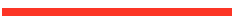
\includegraphics[width=0.1\textwidth]{sepLine}
         \vspace{0.2cm}

	\large
        \begin{center}
		\begin{tabular}{rl}
    			\textbf{Laboratory} & Learning Algorithms and Systems Laboratory (LASA)\\
			\textbf{Professor} & Prof. Aude Billard \\
    			\textbf{Supervisors} & Mahdi Khoramshahi and Andrew Sutcliffe\\
			\textbf{Semester} & Spring 2017\\
		\end{tabular}
	\end{center}
	\vspace{0.05cm}
         \centering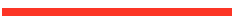
\includegraphics[width=0.1\textwidth]{sepLine}
         \vspace{0.6cm}
         \vfill
\end{titlepage}

	
	\tableofcontents
	
	\chapter{Introduction}
	{
		\section{Motivations}
		{
			\paragraph{} For long and complex tasks, usual machine learning algorithms are often unable to come up with with feasible solutions, or at least fail to do so in acceptable computational times. A natural way to accelerate the learning process is to provide a learning algorithm with prior belief on its environment, as well as recommandations with respect to the task it is trying to learn. 
			
			\paragraph{} Hence, we provide the learning algorithm with demonstrations, much like we would do with a child in the process of learning a skill (dancing, kicking a ball,..). We will use such an example in the following paragraph in order to highlight the different sources of difficulties such an approach might arise.\newline
			Because the teacher doesn't have the same physical abilities than the child, or is not an expert in the skill he is trying to teach, he might give the child a suboptimal way of performing the task. In a ideal learning process, the child would use the prior information given by the teacher, and use it to practice its skill. He will soon be aware of its own abilities, and can then start learning by itself, exploring around the way he has learnt so far. He might find that, by slightly changing how he performs the tasks,  he is able to perform better than the teacher. Therefore, the learning child will first be \emph{compliant} with the teacher, before trying things out by itself once it has become pretty good at performing the learned skill. 
			
			\paragraph{} This semester project aims at introducing a theoretical formulation of such a compliance-based behavior, and experimentally test its performance on simple problems and compare it to other usual algorithm. We will define our problem in a reinforcement learning framework, which allows a fairly good definition of our initial problem. 
			
			\paragraph{} The underlying goal behind this objective is to get better intuition about how interactive learning between human and robots can be achieved. Indeed, we would like to be able to teach a robot from demonstration not by only by providing it a large number of trajectories that he will then use as a motion generator, but by directly interacting with him. By showing a robotic arm, at different times of its learning procedure, concrete examples on how to avoid its closest obstacle and grab a given object, seems like a more natural way of teaching the robot a task, while still enabling him to correct some small sub-optimality we could have introduced to it. 
			
			\paragraph{} Our approach also allows use to tackle a somehow different problem, related to transfer learning. Indeed, the teacher might not be a human but another learner, only better trained than the current learner. In such a case, we would like our learner to quickly find if it can trust its mentor, and if not where it should focus its computations to overcome its mentor sub-optimality. Such questions will therefore be tackled in this report. 
		}
		\section{Background}
		{
			\paragraph{} We hereinafter introduce some notions from the Learning from Demonstration (LfD) framework, as well as some transfer learning metrics that will show useful later on. 
			\subsection{Learning from demonstration}
			{
				\paragraph{} As discussed before, Learning from demonstration (LfD) is a framework where a robot can learns from interacting with a human. It particularly focus on the case where a mentor (human) provides demonstration on how to perform a task. Such an approach is also known as Programming from demonstration (PbD) or imitation learning. 
				
				\paragraph{} LfD mostly lies on the principle that the learning robot can be taught new tasks by end-users, without having to be programmed again. We therefore are dealing with robot that are able to generalize from demonstration, be it only to understand what is the task that they must learn. They are many underlying problematics and opened questions on the subject, detailed in \cite{Billard2016}.
				
				\paragraph{} On approach of LfD combines with reinforcement learning techniques. A could argument for this is that LfD could easily speed-up the learning process by providing a finite or infinite set of good solutions. However, this assume some kind of reproducibility by the robot, as well as a similar enough context between demonstration and reproduction. \newline
				Under such assumptions, RL techniques can use LfD to speed up their learning process and discover new control policies through a directed exploration of its action-state space. Indeed, demonstrations are used to guide the RL algorithm exploration, reducing the time and iterations needed for an agent to discover a new control policy, and eventually overcoming the teacher's apparent policy sub-optimalities. 
				
				\paragraph{} They are many ways of performing such a demonstration-based learning. We remind here a few of them, taken from \cite{argall2009survey}, all related to Imitation Reinforcement Learning (IRL) : 
				\begin{itemize}
					\item policy derivations techniques : directly approximate the robot's mapping from state to action by reproducing and generalizing the teacher's one. 
					\item use demonstration data to learn a model from the world's dynamic (or transition probability model) to compute the optimal policy (see \cite{price2003accelerating}). 
					\item use demonstration data and additional user intention to learn the rule that associate a set of pre and post-condtions which each action as well as a sparse transition model to plan for actions. 
				\end{itemize}
				
				\paragraph{} The framework we described hereinbefore can easily be extended to more than one teacher. Moreover, such teachers can actually be other learning algorithms with different levels of training. Quickly, the problem drifts toward the underlying issue of performing transfer skill between agents. As this will also be tackled during this project, the next section reminds a few useful facts about the theory of transfer learning. 
			}
			\subsection{Transfer learning}
			{
				\paragraph{} Transfer learning deals with speeding a learning process thanks to another learning experience - for instance training an agent based on the previous training on another agent, performing a similar task. The literature of transfer learning in reinforcement learning is pretty large, and for a full description of the different problematics (homogeneous / inhomogeneous sets of actions, multi task learning, ..) we'll refer to \cite{taylor2009transfer}. 
				
				\paragraph{} As we said before, one of our goal is to assess our method as a transfer learning one, and up to a point, consider our teacher to be a trained (fully or not) agent, before considering many different agents as potential mentors. We would consider a really simple case of transfer learning, where all agents display the same state-action state, with the same abilities and constraints. 
				
				\paragraph{} Hence, we remind here some metrics to evaluate transfer learning methods that we would have to use to compare our different approaches : 
				\begin{itemize}
					\item \emph{Jump start} : the initial performance of an agent can be improved by transfer. 
					\item \emph{Asymptotic performance} : how close is the asymptotic learned policy from the optimal policy ? 
					\item \emph{Total or averaged reward} : averaged reward may be improved by transfer 
					\item \emph{Transfer ratio} : Ratio of total reward accumulated by the transfer learner and the total of reward accumulated by a non-transfer learner. 
					\item \emph{Time to threshold} : the time required by a transfer learning to reach a pre-specified level of skills in achieving its task. 
				\end{itemize}
				
				\paragraph{} All those metrics actually compared different aspects of how well a RL algorithm learns. Comparing two RL methods is actually still an open question, and hence we'll need to address several of those metrics to decide on the wellness of our derived TL methods. 
			}
		}
		\section{Proposed approach}
		{
			\paragraph{} A reinforcement learning approach makes a lot of sense in our situation. The next chapter of this report is dedicated to derive some background on this framework, therefore we will hereinafter only describe our proposed approach of imitation learning with a reinforcement learning formulation. 
			
			\paragraph{} In the most general case, we will consider the teacher's demonstrations to be a bijection between the state space $\mathcal{S}$ of the robot and its action set $\mathcal{A}(s)$, $\forall s\in\mathcal{S}$, denoted $\pi_m$ : 
			\begin{equation}
				\begin{aligned}
					\pi_m \, :  \, \mathcal{S} &\to \mathcal{A}\\
						     s &\to a_m(s) 
				\end{aligned}
			\end{equation}
			where $a_m(s)$ is the \emph{recommended action} of the mentor at state $s$. Some other specifications could be brought later on - like considering that the mentor's recommandations don't cover the whole state space, or introducing \emph{inhomogeneous settings}. Given those informations, we want to come up with a learning algorithm that comes up with its own mapping $\pi$, by observing $\pi_m$ and eventually becoming better (we will see later how we define that notion) that its mentor at the demonstrated task. 
			

			\paragraph{} Practically speaking, we are going to start with a fairly simple environment and explicit task in order to address the problem of compliance in learning from a teacher. We hope that a simple enough state space will allow us to better understand how compliance in learning by demonstration should be tackled with a reinforcement learning formulation.  We also hope we would be able to generalize to more complex situations once the understanding on a simple but generic model is mastered. 
			
			\paragraph{} Hence, after defining a simple two dimensional grid-world state space with a simple action set, we will quickly study how well the different classical reinforcement learning policy search algorithms performs on such a space. Once this done, we will introduce a new exploration policy, based on the learned confidence the learner has in its teacher and compare its efficiency with the latter algorithms. We will also focus on the relation between the learner and the prior information on its tasks it gains through its mentors recommandation. Especially, we will study how well a learner can overcome its mentor own sub-optimality. 
		}
	}
	\newpage
	
	\chapter{Reinforcement Learning}
	{
		\section{Formulation}
		{
			\subsection{Notations and first definitions}
			{
				\paragraph{} Reinforcement learning is a framework in which an \emph{agent} (or a \emph{learner}) learns its actions from interaction with its environment. The environment generates scalar values called \emph{rewards}, that the agent is seeking to maximize over time. 
			
				\paragraph{} Let $\mathcal{S}$ denote the state space in which our agent evolves (the localization of a robot on a grid for instance), and $\forall{s}\in\mathcal{S}$ we will define the action state $\mathcal{A}(s)$, describing all possible action that can be taken by the agent at state $s$. When taking an action from a state $s_t$, the agent finds itself in a new state $s_{t+1}$ where it receives a reward $r_{t+1}\in\mathbb{R}$. The action taken is sampled over a probability distribution from the joint space of state and action : 
				\begin{equation}
					\begin{aligned}
						\pi \, : \, \mathcal{S}\times\mathcal{A}(s) \, &\to [0,1]\\
							 (s,a) \, &\to \,  \pi(s,a)
					\end{aligned}
				\end{equation}	
				where $\pi(s,a)$ is the probability of picking action $a$ in state $s$. Such a distribution is called the agent's \emph{policy}. The key goal of reinforcement learning is teaching an agent on how to change its policy to maximize its reward on the long run. 
				
				\paragraph{} The agent indeed seeks to maximize the \emph{expected return} $R_t$ mapping the reward sequence into $\mathbb{R}$. A commonly used expression for this value employs a \emph{discount factor} $\gamma \in [0,1]$, allowing to make the agent's more sensible to rewards it will get in a close future : 
				\begin{equation}
					R_t = \sum_{i=0}^T \gamma^i r_{t+1+i}
				\end{equation}
				This also allows to adapt this formulation to continuous tasks, where there are no terminal states and the task goes on indefinitely (there are no \emph{episodes} in the learning). 
				
				%% TODO : quote Sutton's book 
			}
			\subsection{Markov decision process}
			{
				\paragraph{} To make the problem tractable, we ask for the state signal to comply with Markov's property, hence to be \emph{memory-less}. For instance, we want to be able to write that, in a stochastic environment, $\forall s'\in\mathcal{S}$ : 
				\begin{equation}
					\mathbb{P}\left( s_{t+1}=s' \, \vert \, a_t, s_t, \hdots, a_1,s_1\right) = \mathbb{P}\left( s_{t+1}=s' \, \vert \, s_t, a_t\right)
				\end{equation}
				
				\paragraph{} Hence, every reinforcement learning problem can be represented by a \emph{Markov Decision Process}, that consists in a 5-tuple $\left(\mathcal{S}, \mathcal{A}, \mathcal{P}_{\cdot}(\cdot,\cdot), \mathcal{R}_{\cdot}(\cdot), \gamma \right)$ where : 
				\begin{itemize}[label=$\triangleright$]
					\item $\mathcal{S}$ is the agent's state space
					\item $\mathcal{A}$ is the agent's action space
					\item $\forall s,s'\in\mathcal{S}, \, \forall a\in\mathcal{A}(s)$,  $\mathcal{P}_a(s,s') = \mathbb{P}(s_{t+1}=s'\, \vert \, s_t = s, a_t = a)$ is the probability that action $a$ in state $s$ will lead the agent to transitioning to state $s'$.
					\item $\forall s,s'\in\mathcal{S}, \, \forall a\in\mathcal{A}(s)$,  $\mathcal{R}_a(s,s')$ is the immediate reward perceived by the agent when transitioning from state $s$ to $s'$ when taking action $a$. 
					\item $\gamma$ is the discount factor. 
				\end{itemize}
				
				\paragraph{} A \emph{finite Markov decision process} designates a MDP for which both the action and state space are finite. 
			}
			\subsection{State and action value function}
			{
				\paragraph{} Most of the reinforcement learning algorithms are based on evaluation value function. A value function is a function mapping the state space in $\mathbb{R}$, estimating how good (in terms of expected future reward) it is for the agent to be in a given space. More precisely, a value function $V^\pi(\cdot)$ evaluates the expected return of a state when following the policy $\pi$. $V^\pi(\cdot)$ is called the \textbf{state-value function}. 
				\begin{equation}
					\forall{s}\in\mathcal{S}, \quad V^\pi(s) = \E[\pi]{R_t \, \vert \, s_t = s}
				\end{equation}
				The \textbf{action-value function} evaluates the value of taking a given action, and then following the policy $\pi$ : 
				\begin{equation}
					\forall{s,a}\in\mathcal{S}\times\mathcal{A}(s), \quad Q^\pi(s,a) = \E[\pi]{ R_t \, \vert \, s_t=s, \, a_t=a}
				\end{equation}
				
				\paragraph{} Both those functions satisfy particular recursive relationships known as the \emph{Bellman equations}. It is shown that (see TODO quote Sutton) we have the following results : 
				\vspace{10pt}
				
				\coolbox{white}{\textcolor{black}{Bellman equations for Markov Decision Process}}
				{
					\begin{itemize}[label=$\triangleright$]
						\item Bellman equation for the state-value function : $\forall s \in\mathcal{S}$ 
						\begin{equation}
							V^\pi(s) = \sum_{a\in\mathcal{A}}\pi(s,a)\sum_{s'} \mathcal{P}_a(s,s')\left[\mathcal{R}_a(s,s') + \gamma V^\pi(s')\right]
						\end{equation}
						\item Bellman equation for the action value function : $\forall{s,a}\in\mathcal{S}\times\mathcal{A}(s)$ : 
						\begin{equation}
							Q^\pi(s,a) = \sum_{s'}\mathcal{P}_a(s,s')\left[ \mathcal{R}_a(s,s') + \gamma V^\pi(s')\right]
						\end{equation}
					\end{itemize}
				}
			}
			\subsection{Optimal policies}
			{
				\paragraph{} The value functions define a partial ordering in the policy space. A policy $\pi$ is therefore said to be better than $\pi'$ (or $\pi\geq \pi'$) if $\forall{s}\in\mathcal{S}$, $V^\pi(s) \geq V^\pi(s')$. We are looking for $\pi^*$ so that : 
				\begin{equation}
					\forall\pi, \quad \pi^* \geq \pi 
				\end{equation}
				
				TODO quote showed that for finite MDPs, there is always at least one policy that is better our equal to all others, and therefore is called the \emph{optimal policy} $\pi^*$. As shown in TODO quote, the state-value and action-value function verify the \emph{Bellman optimality equations}. 
				
				\vspace{10pt}
				
								\coolbox{white}{\textcolor{black}{Bellman optimality equations}}
				{
					\begin{itemize}[label=$\triangleright$]
						\item Bellman optimality equation for the state-value function : $\forall s \in\mathcal{S}$ 
						\begin{equation}
							V^\pi(s) = \max_{a\in\mathcal{A}(s)}\pi(s,a)\sum_{s'} \mathcal{P}_a(s,s')\left[\mathcal{R}_a(s,s') + \gamma V^\pi(s')\right]
						\end{equation}
						\item Bellman optimality equation for the action value function : $\forall{s,a}\in\mathcal{S}\times\mathcal{A}(s)$ : 
						\begin{equation}
							Q^\pi(s,a) = \sum_{s'}\mathcal{P}_a(s,s')\left[ \mathcal{R}_a(s,s') + \max_{a\in\mathcal{A}(s')} Q(s',a') \right]
						\end{equation}
					\end{itemize}
				}
				
				\paragraph{} Those relations are essential in understanding the solving algorithms that will be presented later. 
			}
		}


			\paragraph{} There exists several ways of solving (i.e computing the optimal policy) of a Markov Decision Process, that can generically be separated in two categories : \emph{model-based} and \emph{model-free} methods. 
		\section{Dynamic Programing}
		{
			\paragraph{} Dynamic programing is a mathematically well-developed theory. It requires the complete and accurate model of the environment, making it a model-based method. 
			
			\paragraph{} Dynamic programing methods aims at computing the optimal value function at every state of state space. This could, of course, be done by solving the $\vert \mathcal{S} \vert $ equations of $\vert \mathcal{S} \vert $ unknowns that are the Bellman equations for a given policy, and then evolve that policy toward a better one, based on the current value function. Of course, this approach is computationally intractable for large state space and therefore needs to be adapted, but gives a first approach of the idea behind dynamic programing. 
				
			\subsection{Generalized policy iteration}
			{
				\paragraph{} The generalized policy iteration methods rely on alternating two processes, known as \textcolor{red}{policy evaluation} and \textcolor{red}{policy improvement}. 
				\begin{itemize}[label=$\triangleright$]
					\item Policy evaluation deals with estimating the value function of a given policy $\pi$, without directly solving the full system given by Bellman equations. The idea is actually pretty simple : use Bellman's equation as an update rule, using that the value function is a fixed point for this update rule. The algorithm, after setting the tabled value function to an initial value, iterate by performing what is called \emph{full Bellman backups} : 
					\begin{equation}
						\forall{s}\in\mathcal{S}, \quad V_{k+1}^\pi(s) = \sum_{a\in\mathcal{S}} \pi(s,a)\sum_{s'}\mathcal{P}_a(s,s') \left[\mathcal{R}_a(s,s')+V_k^\pi(s')\right]
					\end{equation}
					This algorithm converges under the same assumptions that guarantee the existence of the value function, and has the generic name of \emph{iterative policy evaluation}. They are many refining for speeding up that process (reduced backups, prioritized sweeping) that we won't address here. 
				\item Policy evaluation is a process that from a given policy value function, returns a better or equal policy compared to the latter. The simplest way to do that is for every state $s\in\mathcal{S}$, consider every action-value functions : 
				\begin{equation}
					Q(s,a) = \sum_{s'}\mathcal{P}_a(s,s')\left[\mathcal{R}_a(s,s') + \gamma V\pi(s')\right], \quad a\in\mathcal{A}(s)
				\end{equation}
				and to build $\pi'$ to be \emph{greedy} with respect to those actions-values : 
				\begin{equation}
					\pi'(s) = \argmax{a\in\mathcal{A}(s)}{Q(s,a)}
				\end{equation}
					The policy improvement theorems then ensures that $\pi'\geq \pi$. 
				\end{itemize}
				
				\paragraph{} Hence, generalized policy improvement are a set of methods that iteratively combine those two sub-methods to compute the optimal policy for a given MDP. Of course, one does not have to perform all sweeps of value evaluation before improving the policy to converge toward an optima (indeed, many times our sweeps won't have any affect on the greedy policy). They are many ways to combine the two (prioritized sweeping, asynchronous dynamic programing), but the most used and one of the most quickest way to converge is to use the value iteration algorithm. 
			}	
			\subsection{The value iteration algorithm}
			{
				\paragraph{} The value iteration algorithm takes the limit of the behavior we just described, and stops the value evaluation procedure after only \emph{one state space sweep}. It therefore performs a simple backup procedure : 
					\begin{equation}
						\forall{s}\in\mathcal{S}, \quad V_{k+1}  = \max_{a\in\mathcal{A}}  \sum_{s'}\mathcal{P}_a(s,s')\left[\mathcal{R}_a(s,s') + \gamma V_k^\pi(s')\right]
					\end{equation}
					For any arbitrary $V_0$, it is shown that $V_k\to V^*$ as $k\to\infty$, under the same hypothesis that ensure the existence of the optimal value function $V^*$. As one can notice, it actually implements the \emph{Bellman optimality conditions} as an update rule !
				}
			}
		
		
		\section{Temporal differences methods}
		{
			\paragraph{} Temporal difference methods can be seen as a combination of dynamic programing and another kind of learning called Monte Carlo methods, where the expected return are approximated via sampling. Like dynamic programming, TD methods are said to bootstrap (meaning that they build their estimators through already estimated values), but are \emph{model-free} methods and learn from experience. 
			
			\paragraph{} The justification, proof of convergences and literature and those models is pretty wide, hence we will not cover them in this report. However, full description of those methods can be found in TODO quote. 
			
			\subsection{On-policy method : SARSA}
			{
				\paragraph{} The SARSA algorithm is an \emph{on-policy} control method, meaning that the algorithm updates the value function and improves the current policy it is following. At state $s_t$, it chooses an action $a_t$ from its policy and follows it. After observing the reward $r_{t+1}$ and the next state $s_{t+1}$, it again chooses an action $a_{t+1}$ using a soft policy and performs a one-step backup : 
				\begin{equation}
					Q(s_t,a_t) \leftarrow Q(s_t,a_t) + \alpha\left[r_{t+1} + \gamma Q(s_{t+1},a_{t+1}) - Q(s_t,a_t)\right]
				\end{equation}
				It therefore relies on a 5-tuple $(s_t,a_t,r_{t+1},s_{t+1},a_{t+1})$ to perform the udpate, giving it the State Action Reward State Action (SARSA) name. 
				\vspace{10pt}
				
				\coolbox{white}{\textcolor{blue}{The General Sarsa Algorithm}}
					{
						\begin{algorithm}[H]
	 					\SetAlgoLined
						\LinesNumbered
						\emph{\textsf{1. Initialize}} $Q(s,a)$ arbitrarily $\forall (s,a)\in\mathcal{S}\times\mathcal{A}(s)$ \\
						\BlankLine
						\BlankLine
						\emph{\textsf{2. Repeat}} for each episode : \\
						\Indp \Indp 
							Initialize $s$ \\
							Choose $a\in\mathcal{A}(s)$ using a soft policy derived from $Q$ (typically $\varepsilon$-greedy) \\
							Repeat for each step of the current episode :   \\
							\Indp \Indp 
								Take $a$, observe $r,s'$ \\
								Choose $a'$ from $s'$ using policy derived from $Q$ 
								$ Q(s,a) \longleftarrow Q(s,a) + \alpha\big[ r + \gamma Q(s',a') - Q(s,a) \big]$ \\
								$a\leftarrow a'$, $s\leftarrow s' $ \\
								
							\Indm \Indm 
						until $s\in\mathcal{S}^+$.
						\Indm \Indm 
						\end{algorithm}
					}
					
					\paragraph{} The convergence properties of SARSA depend on the nature of the policy's dependency on Q. Indeed, SARSA converges with probability 1 to the optimal policy as long as all the sate and actions pairs are visited an infinite number of time, and the policy converges in the limit to the greedy policy. This is done, for instance, by turning the temperate of a softmax based policy to 0, or by having $\eps\to 0$ for a $\eps$-greedy policy. For SARSA to converge, we also as the learning rate to comply with the stochastic approximation conditions : 
					\begin{equation}
						\sum_k \alpha_k(a) = +\infty \quad { and } \quad \sum_k \alpha_k(a)^2 < +\infty
					\end{equation}
					where $\alpha_k(a)$ is the learning rate for the k\textsuperscript{th} visit of the pair $(s,a)$. 
					
			}
			\subsection{Off-policy method : Q-learning}
			{
				\paragraph{} The Q-learning algorithm is an off-policy method who learns to directly approximate $Q^*$, independently of the policy being followed. Its update rule is given by :
				\begin{equation}
					Q(s_t,a_t) \leftarrow Q(s_t,a_t) + \alpha \left[ r_{t+1} + \gamma \max_{a\in\mathcal{A}(s_{t+1})} Q(s_{t+1},a) - Q(s_t,a_t)\right]
				\end{equation}
				The actual policy being followed still has an effect in that it determines which state-actions pairs are visited and updated. However all that is required for convergence it that all pairs continue to be updated. 
				\vspace{10pt}
				
				\coolbox{white}{\textcolor{blue}{Q-Learning Algorithm}}
					{
						\begin{algorithm}[H]
	 					\SetAlgoLined
						\LinesNumbered
						\emph{\textsf{1. Initialize}} $Q(s,a)$ arbitrarily $\forall (s,a)\in\mathcal{S}\times\mathcal{A}(s)$ \\
						\BlankLine
						\BlankLine
						\emph{\textsf{2. Repeat}} for each episode : \\
						\Indp \Indp 
							Initialize $s$ \\
							Repeat for each step of the current episode :   \\
							\Indp \Indp 
								Choose $a\in\mathcal{A}(s)$ using arbitrary policy \\
								Take $a$, observe $r,s'$ \\
								$ Q(s,a) \longleftarrow Q(s,a) + \alpha\big[ r + \gamma \max_{a'\in\mathcal{A}(s')}Q(s',a') - Q(s,a) \big]$ \\
								$s\leftarrow s' $ \\
								
							\Indm \Indm 
						until $s\in\mathcal{S}^+$.
						\Indm \Indm 
						\end{algorithm}
					}
				
				\paragraph{} Along with this hypothesis and a slight variation in the usual stochastic approximation conditions, the learned action value function by Q-learning has been shown to converge to $Q^*$ with probability $1$. 
			}
			\subsection{Eligibility traces}
			{
				\paragraph{} In TD(0) approach (described in the latest section), we update the value function in the direction of the \emph{one-step return} : 
				\begin{equation}
					\Delta V_t(s_t)^{(1)} = \alpha \left[ r_t + \gamma V_t(s_{t+1}) - V_(s-t)\right]
				\end{equation}
				The idea behind eligibility traces is to expand that update rule in order to steer the value fonction towards the \emph{n-step return} (or at least until a terminal state is reached) :
				\begin{equation}
					\begin{aligned}
					\Delta V_t(s_t) ^{(n)} &= \alpha \left[ r_t + \gamma r_{t+1} + \hdots + \gamma^{n} V_t(s_{t+n})-V_t(s_t)\right]	\\
									&= \alpha \left[R_t^{(n)} - V_t(s_t)\right]
					\end{aligned}
				\end{equation}
				
				\paragraph{} The backups can not only be done toward any n-step return, but toward any average of such returns, as long as the corresponding weights sum-up to one. In this way, the TD($\lambda$) algorithm can be understood as a particular way of averaging $n$-steps returns. With $\lambda<1$, the resulting backup is known as the \textcolor{red}{\emph{$\lambda$-return}} : 
				\begin{equation}
					R_t^\lambda = (1-\lambda) \sum_{n=1}^\infty \lambda^{n-1}R_t^{(n)}
				\end{equation}
				where the weights are fading with $n$. When the runs are episodic, we can write this return as : 
				\begin{equation}
					R_t^\lambda = (1-\lambda)\sum_{n=1}^{T-t-1} \lambda^{n-}R_t{(n)} + \lambda_{T-t-1}R_t^{(T)}
				\end{equation}
				
				\coolbox{white}{\textcolor{blue}{Sarsa($\lambda$) algorithm}}
					{
						\begin{algorithm}[H]
						\label{sarsalambda}
	 					\SetAlgoLined
						\LinesNumbered
						\emph{\textsf{1. Initialize}} $Q(s,a)$ arbitrarily $\forall (s,a)\in\mathcal{S}\times\mathcal{A}(s)$ \\
						\BlankLine
						\BlankLine
						\emph{\textsf{2. Repeat}} (for each episode) : \\
						\Indp \Indp 
							Initialize $s,\, a$ \\
							Repeat for each step of the current episode :   \\
							\Indp \Indp 
								Take action $a$, observe $r, s'$. \\
								Choose $a'\in\mathcal{A}(s')$ using soft policy derived from $Q$\\
								$\delta \longleftarrow r + \gamma Q(s',a') - Q(s,a)$ \\
								$e(s,a) \longleftarrow e(s,a) +1 $\\
								For all $s,a$ : \\
								\Indp \Indp 
									$ Q(s,a) \longleftarrow Q(s,a) + \alpha \delta e(s,a) $ \\
									$ e(s,a) \longleftarrow \gamma \lambda e(s,a) $\\
								\Indm \Indm 
								$s\leftarrow s'$, $a\leftarrow a'$\\						
							\Indm \Indm 
						until $s\in\mathcal{S}^+$.\\
						\Indm \Indm 
						\end{algorithm}
					}


				\paragraph{} Such a formulation of eligibility traces is known as the \emph{\textcolor{red}{forward view}} of TD($\lambda$), and shows how eligibility traces build the bridge between TD(0) methods and Monte-Carlo one. It is not implementable as is since it is non-causal. There exist a more mechanistic view, equivalent to the forward view (see \cite{Sutton98a}), known as the \emph{backward-view}. It gives birth to causal version of the TD($\lambda$) method. We give as an example the pseudo-code for the SARSA($\lambda$) algorithm above. Its Q-learning equivalent can be found in \cite{Sutton98a}.   
			}
		}
	
		\section{Grid-world examples}
		{
			\paragraph{} We hereinafter describe two grid-world space, on which we will apply the learning rule derived in the latest section. Such example are trivial and are displayed here just to show convergence and behavior of the different algorithms. 
			
			\paragraph{} We'll consider the two following state space : 
			\begin{figure}[h!]
				\begin{minipage}{0.45\linewidth}
					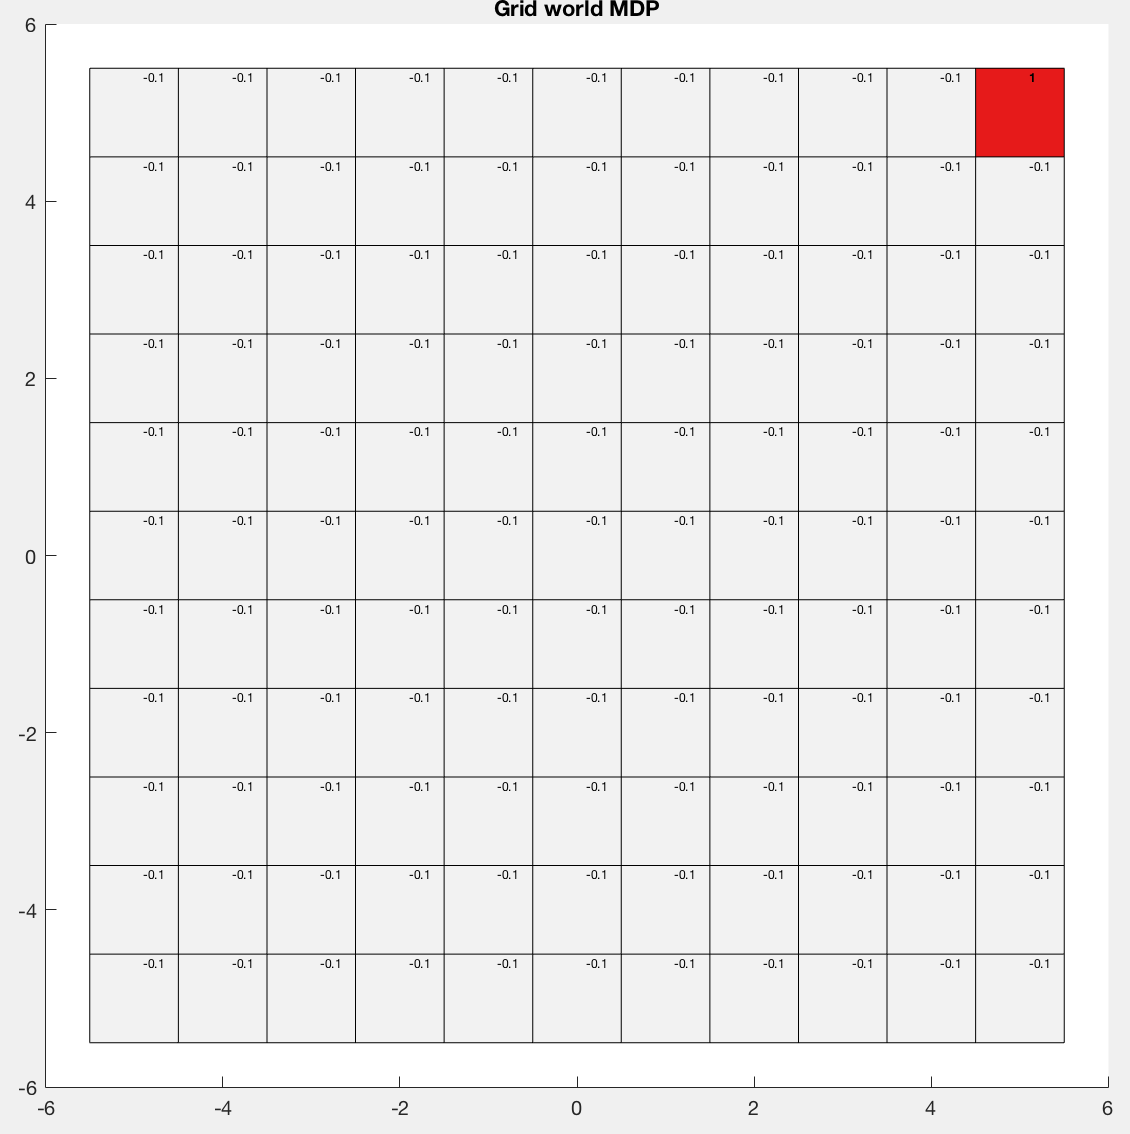
\includegraphics[width=\linewidth]{free_grid}
					\caption{The \emph{free\_grid} state space}
				\end{minipage}
				\hfill
				\begin{minipage}{0.45\linewidth}
					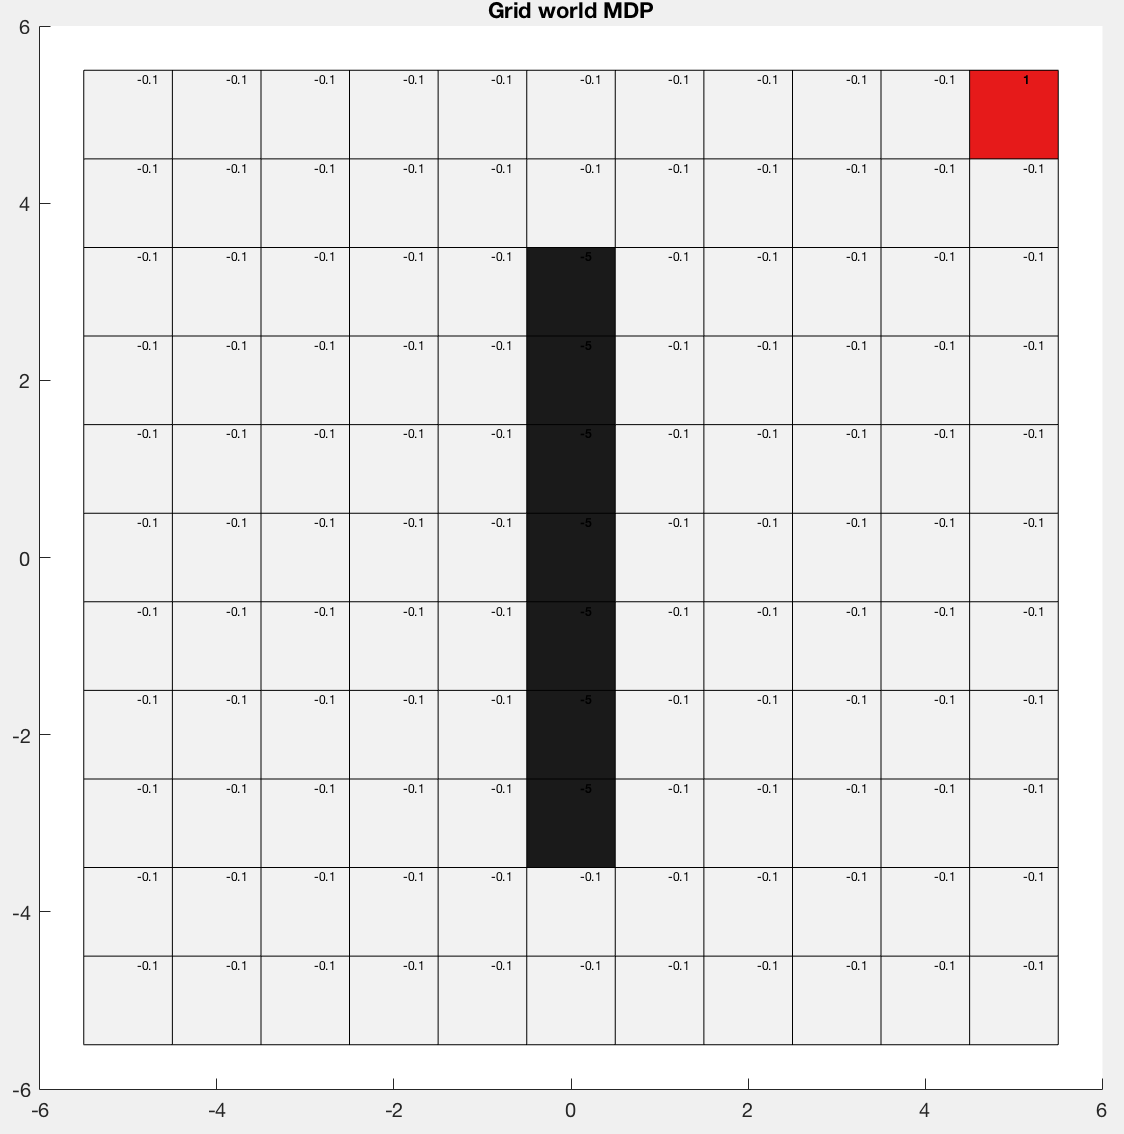
\includegraphics[width=\linewidth]{bar_grid}
					\caption{The \emph{bar\_grid} state space}
				\end{minipage}
			\end{figure}
			\subsection{Dynamic Programing solving}
			{
				\paragraph{} Let us run the DP algorithm on such grid worlds. We'll consider a stochastic environnement, with the transition probability : 
				\begin{equation}
					\mathcal{P}_{s,s'}^a = \left\{\begin{aligned} &0.9 &\text{ if }s' = s(a) \\ &0.1 &\text{ otherwise} \end{aligned}\right.
				\end{equation}
				Running the value iteration algorithm (assuming we now the environment model), we obtain the following policies and learning curves. The stopping criterion adresses the maximum absolute change brought to the value function as the sweeping goes through the state space : 
				\begin{equation}
					\text{ If } \max_{s\in\mathcal{S}} \vert V_{k+1}(s) - V_k \vert < \delta \text{ then stop}
				\end{equation}
				
				\begin{figure}[h!]
				\begin{minipage}{0.45\linewidth}
					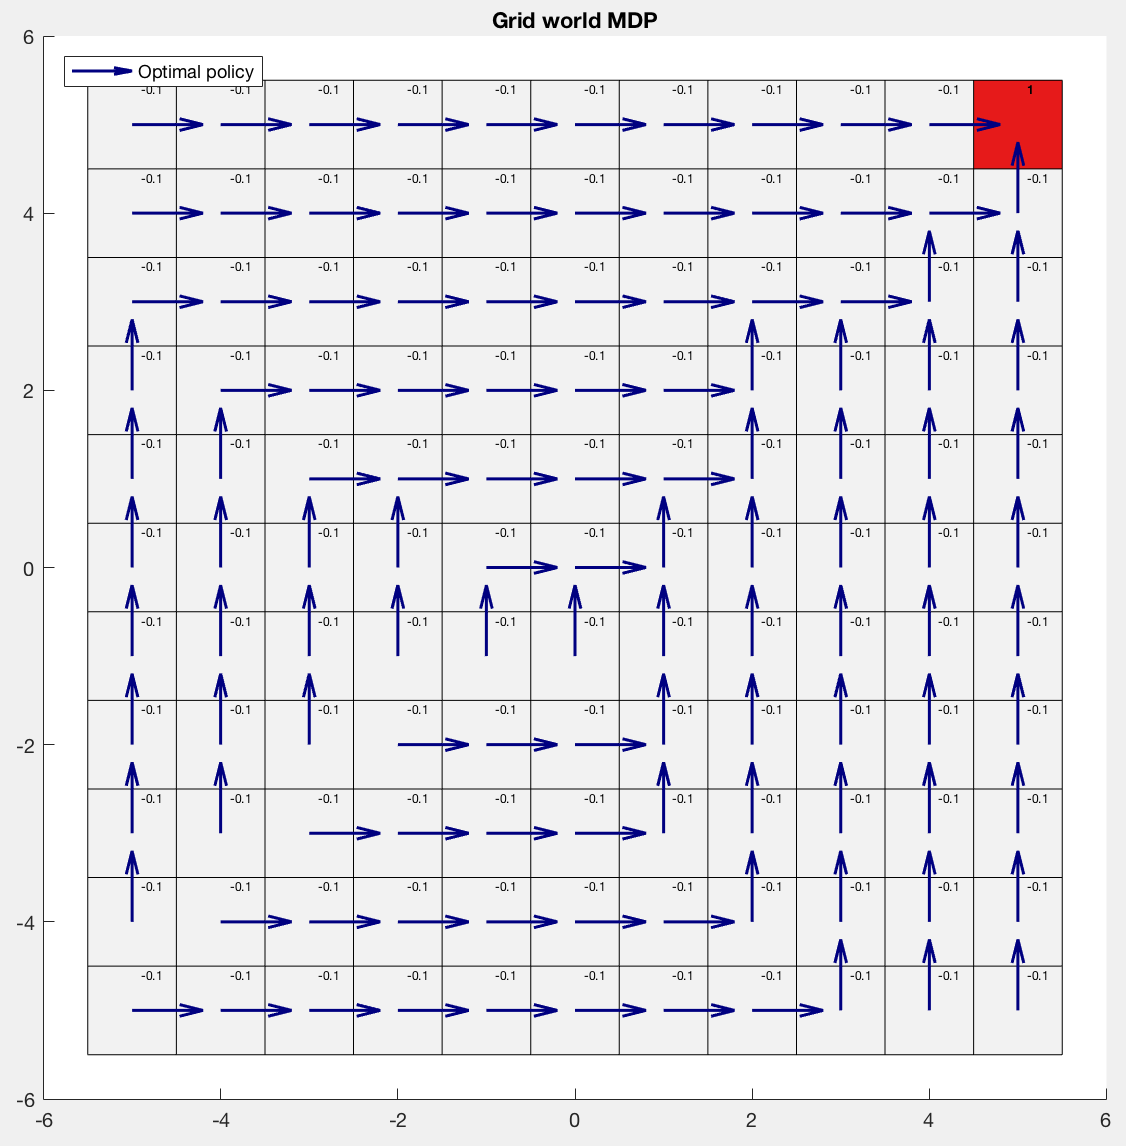
\includegraphics[width=\linewidth]{free_grid_bellman_policy}
					\caption{The \emph{free\_grid} learned optimal policy}
				\end{minipage}
				\hfill
				\begin{minipage}{0.45\linewidth}
					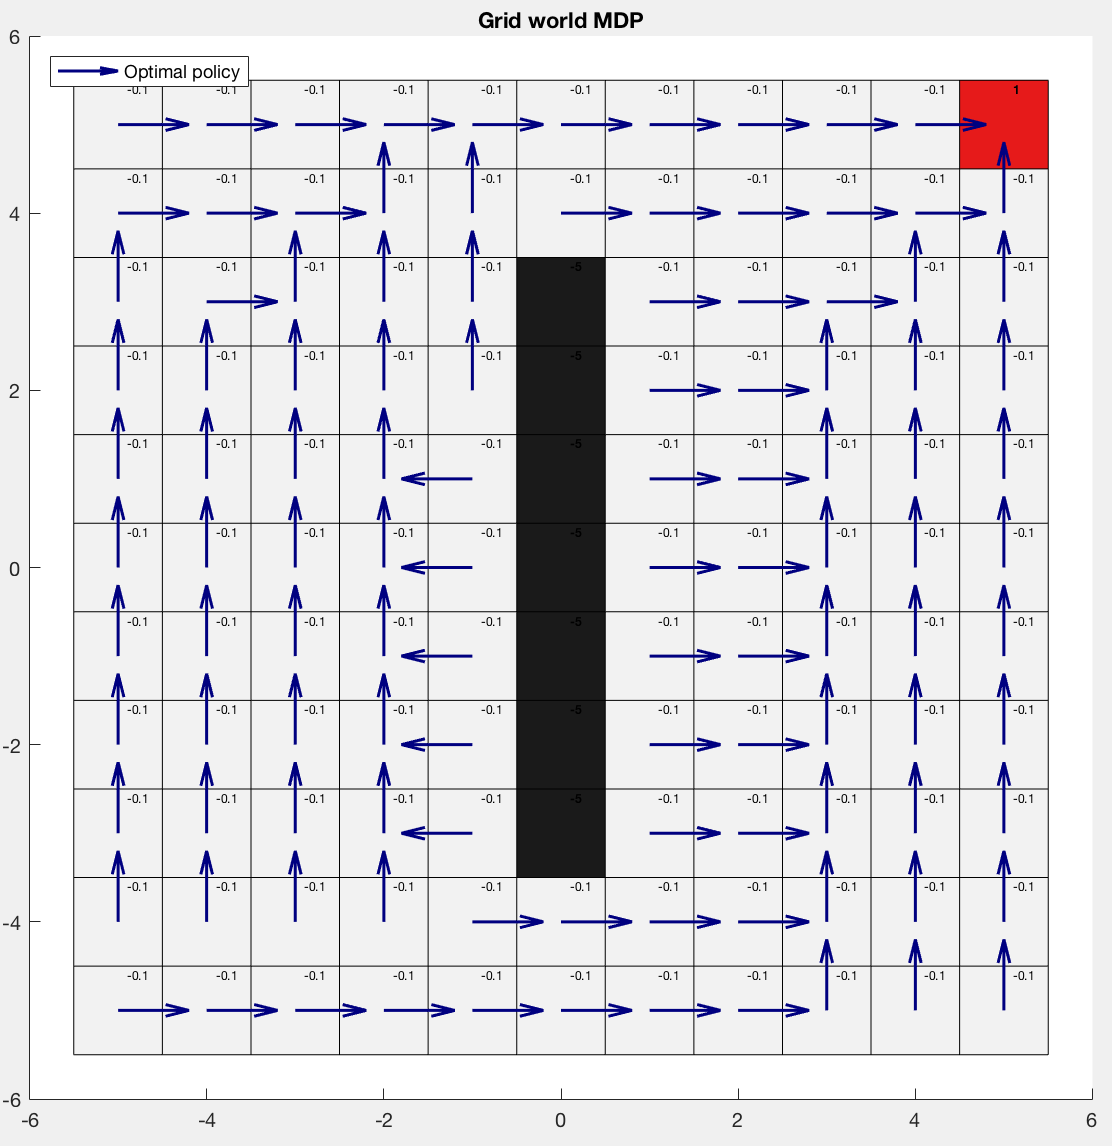
\includegraphics[width=\linewidth]{bar_grid_bellman_policy}
					\caption{The \emph{bar\_grid} learned optimal policy}
				\end{minipage}
				\end{figure}
				
				\begin{figure}[h!]
				\begin{minipage}{0.45\linewidth}
					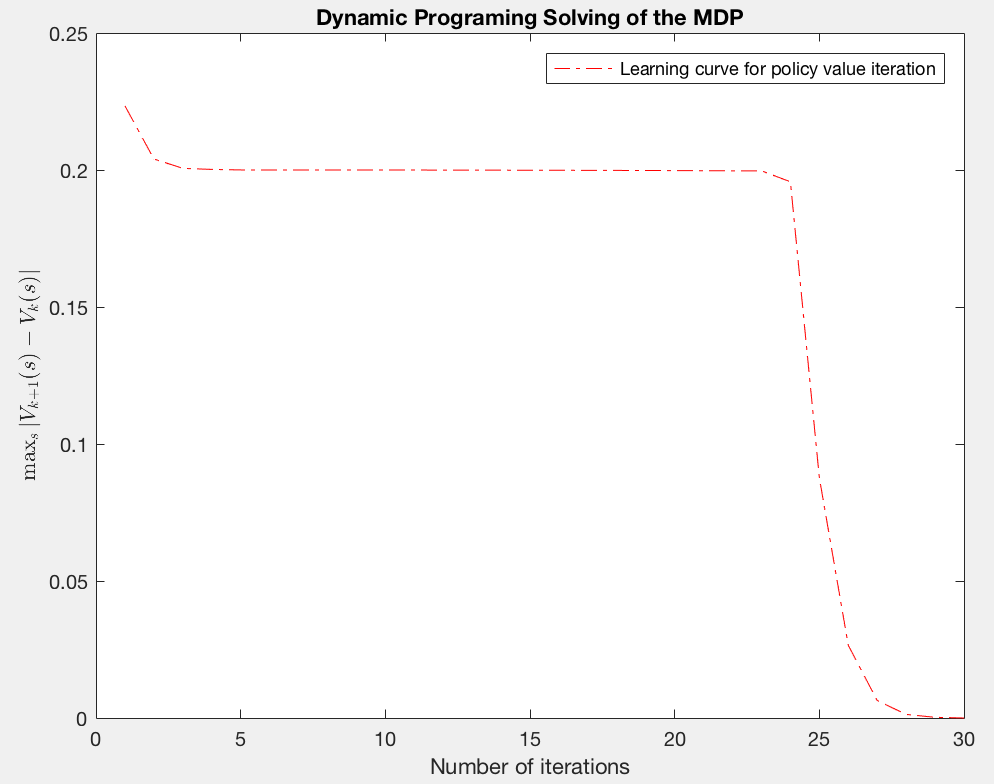
\includegraphics[width=\linewidth]{free_grid_bellman_lc}
					\caption{The \emph{free\_grid} value iteration learning curve}
				\end{minipage}
				\hfill
				\begin{minipage}{0.45\linewidth}
					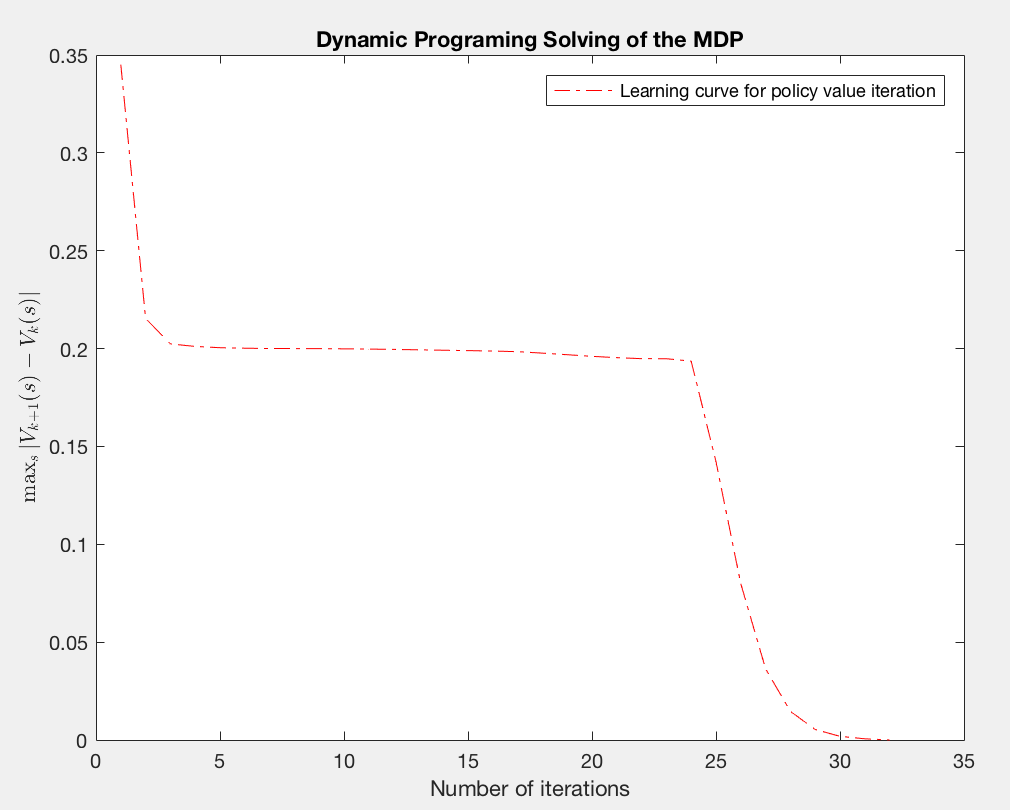
\includegraphics[width=\linewidth]{bar_grid_bellman_lc}
					\caption{The \emph{bar\_grid} value iteration learning curve}
				\end{minipage}
				\end{figure}
				
				\paragraph{} One can notice that for the \emph{bar\_grid} environment, the agent undergoes a longer trajectory than necessary, at the left of the obstacle. This is because of the stochastic nature of the environment, causing the agent to learn to takes its distance with the obstacle in order not to accidentally hit it (and then receive a very negative reward). 
				
				\paragraph{} The learned policy are indeed optimal. The next algorithms (SARSA and Q-learning) will try to reproduce them without a model for the environment. 
			}
			\subsection{SARSA solving}
			{
				\paragraph{} We display here the learning curves for the \emph{free\_grid} state space using SARSA. The algorithm manages to learn the optimal policy and the right action-value functions. We use \emph{optimistic initialization} to encourage exploration, and Gibbs sampling for following a soft-policy : $\forall (s,a) \in\mathcal{S}\times \mathcal{A}(s)$ 
				\begin{equation}
					\pi(s,a) = \displaystyle \frac{ e^{Q(s,a)/\tau}}{\sum_{a'\in\mathcal{A}(s)}e^{Q(s,a')/\tau}}
				\end{equation}
				We'll tune the distribution's temperature $\tau$ to zero, in order to converge toward the greedy policy w.r.t the learned action-value function. 
				
				\paragraph{} Following this strategy and tuning our learning rate to comply with the stochastic approximation conditions, we obtain the following learning curves. Again, our stopping criterion addresses the \emph{maximum change in the acton-value function over all the trajectories of a mini-batch}. 
				\begin{figure}[h!]
					\begin{minipage}{0.4\linewidth}
						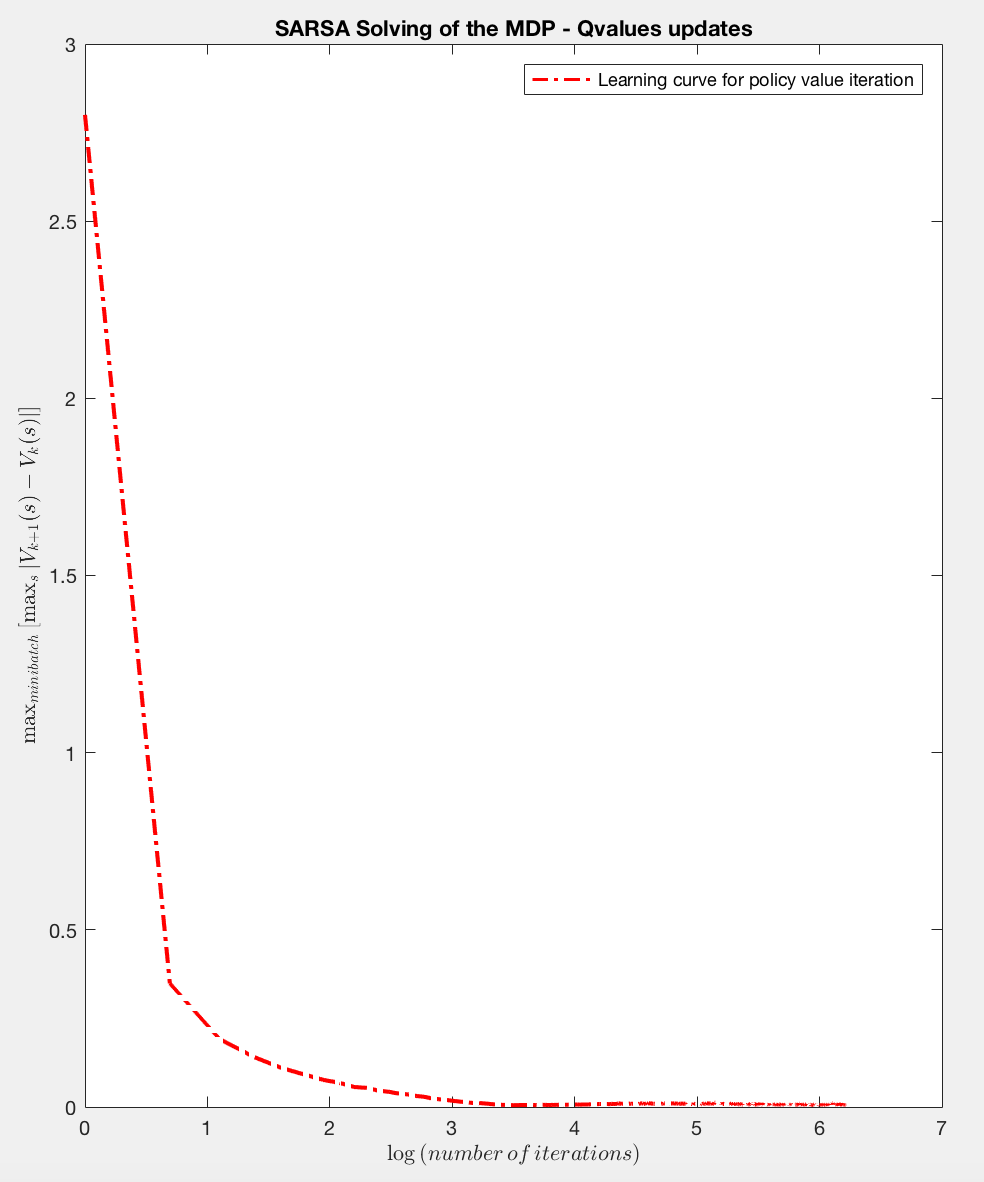
\includegraphics[width=\linewidth]{sarsa_learning_curve_free_grid}
						\caption{Learning curve for SARSA on \emph{free\_grid}}
					\end{minipage}
					\hfill
					\begin{minipage}{0.4\linewidth}
						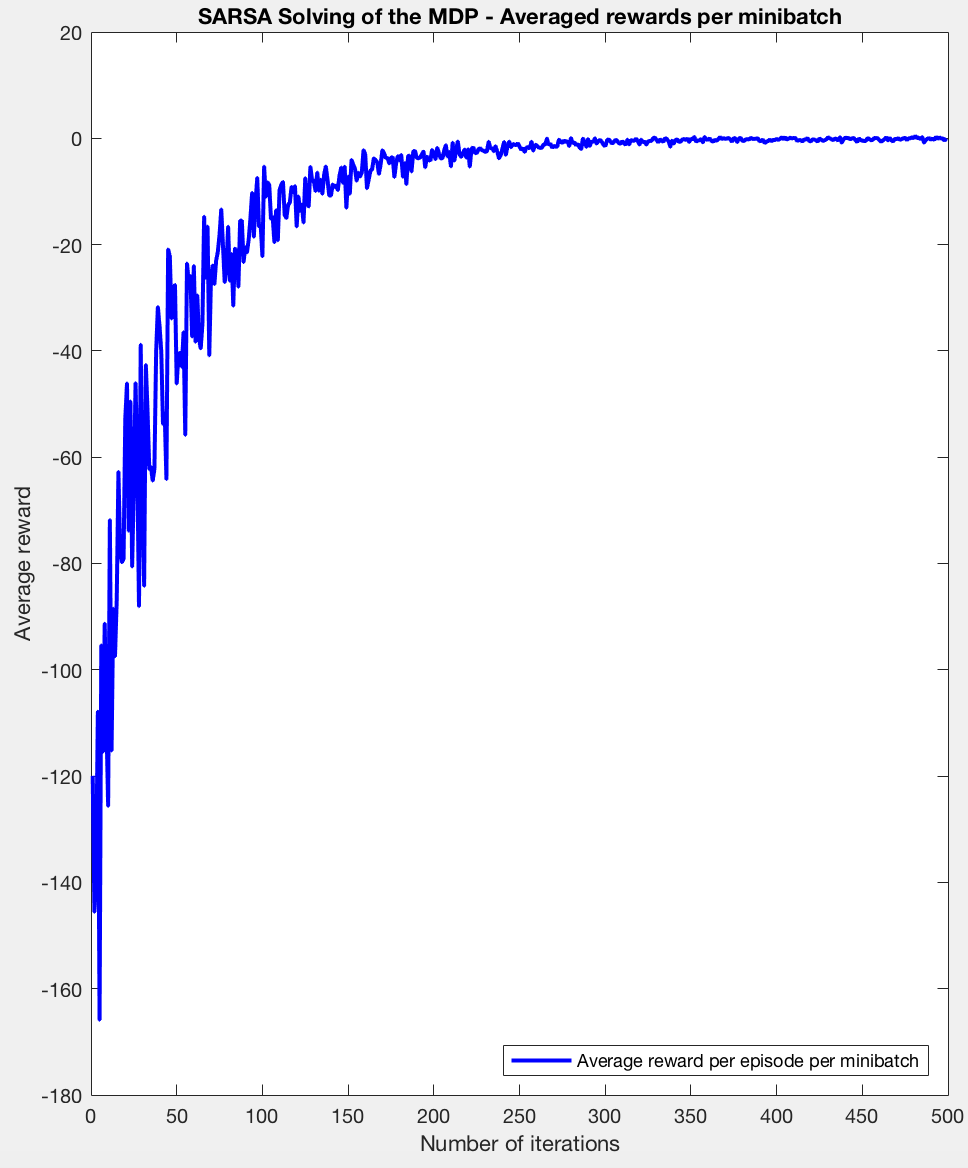
\includegraphics[width=\linewidth]{sarsa_average_rewards_freegrid}
						\caption{Averaged rewards over mini-batch for SARSA on \emph{free\_grid}}
					\end{minipage}
				\end{figure}
				  
			}
			\subsection{Q-learning solving}
			{
				\paragraph{} We display here the learning curves for the \emph{bar\_grid} state space using Q-learning. Again, the algorithm manages to learn the optimal policy and the right action-value functions. We use Gibbs sampling for the behavior policy, without any tuning for the temperature (the behavior policy doesn't need to be greedy in limit). The learning curves obtained are given hereinafter.
				\begin{figure}[h!]
					\begin{minipage}{0.4\linewidth}
						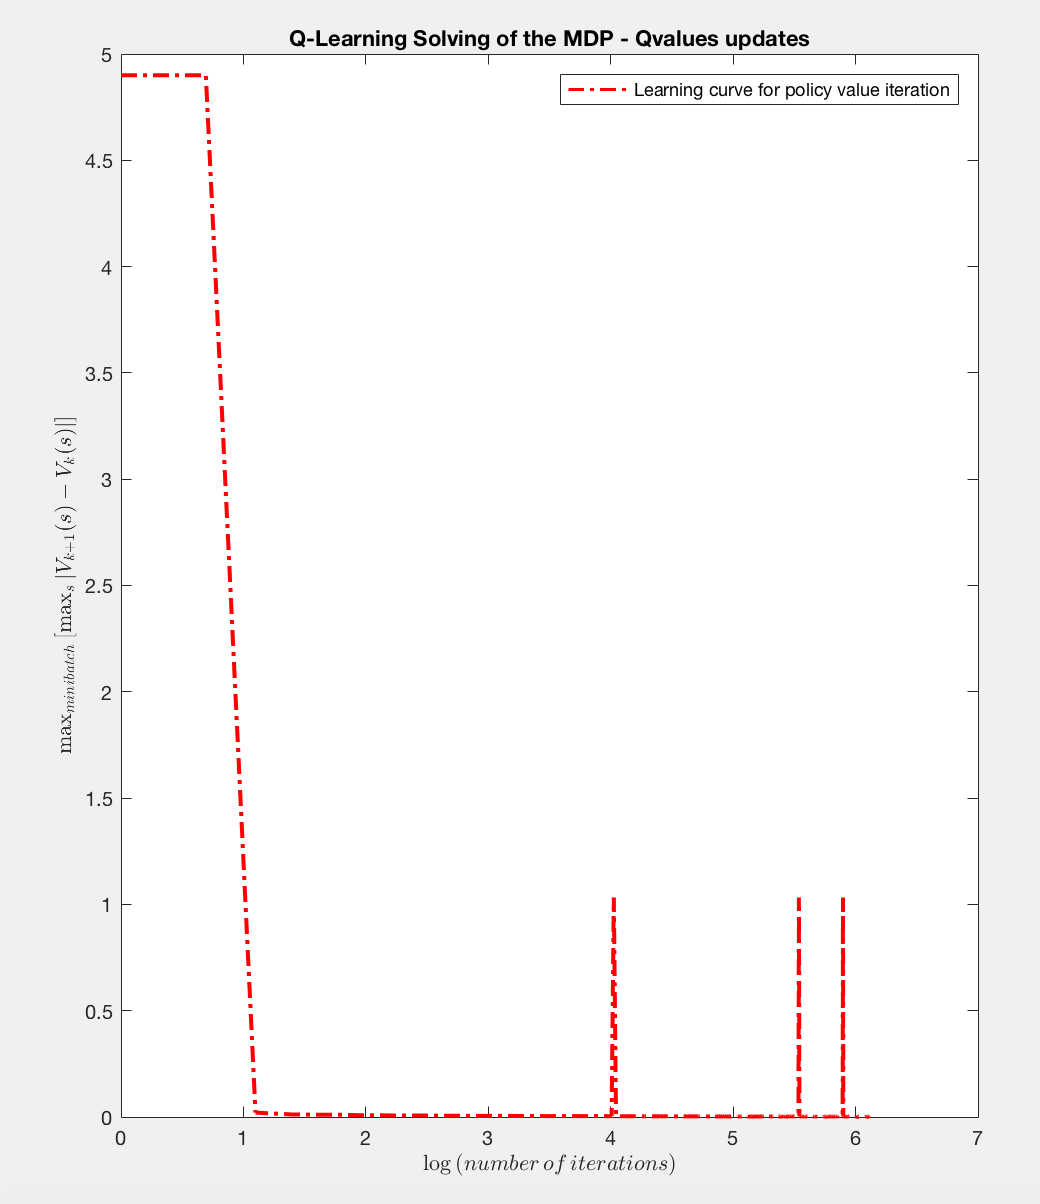
\includegraphics[width=\linewidth]{bargrid_ql_learning_curve}
						\caption{Learning curve for Q-learning on \emph{bar\_grid}}
					\end{minipage}
					\hfill
					\begin{minipage}{0.4\linewidth}
						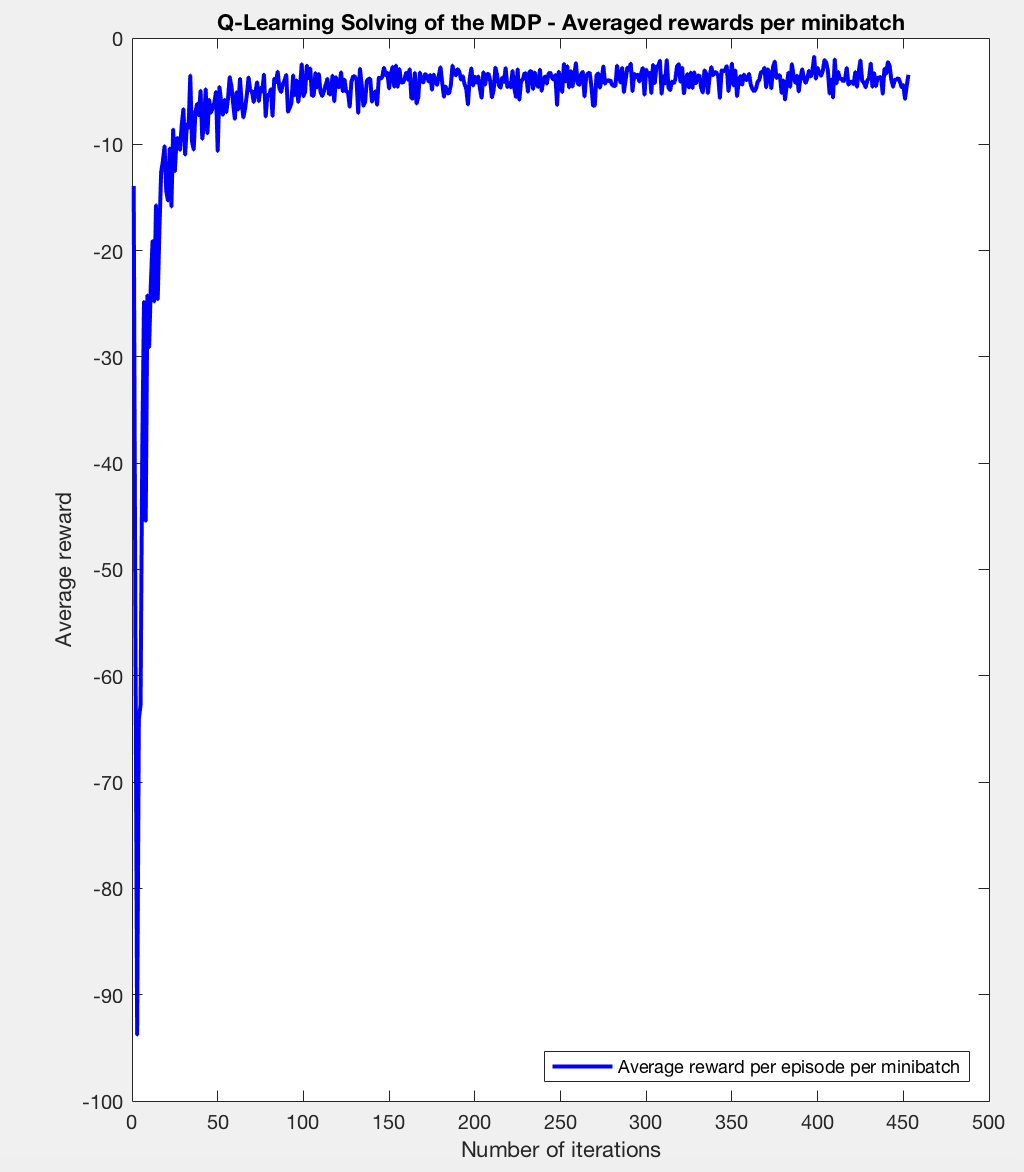
\includegraphics[width=\linewidth]{bargrid_ql_averaged_rewards}
						\caption{Averaged rewards over mini-batch for Q-learning on \emph{bar\_grid}}
					\end{minipage}
				\end{figure}

			}
		}
	}
	
	\chapter{Compliant-based reinforcement learning}
	{
		\section{Problem selection}
		{
			\paragraph{} With our approach, we wish to tackle two topics : on one hand, we wish to display a imitation based learning framework that \emph{accelerate} the learning process. Also, we wish to have a shifting compliance based behavior so that an agent can \emph{overtake a suboptimal teacher}. To test the effectiveness of the solutions we would propose, we decided to provide ourself with a model that would stay fixed all along the experiments, in order to compare the different algorithms we could come up with. 
			
			\paragraph{} We therefore needed to provide an environment that, with the algorithms described before, cannot solve its MDP quickly, and can sometimes get stuck in local minima. We chose the state space displayed in figure (\ref{fig::maze_display}). In this environment, all black cells are obstacles. They give out highly negative rewards ($r=-10$). Whenever an agent take the action to enter such a cell, it immediately perceives the negative reward but stays in its current cell. The only positive reward in this environment is at the middle of the grid ($r=10$), the only terminal state. Any trajectory of the learner starts at one of the corner of the grid (green cells), and every step spent on a non-terminal cell gives out a small negative reward ($r=-0.1$). The environment is stochastic, with the transition probability model : 
			\begin{equation}
				s' = \left\{ 
					\begin{aligned}
						&a(s) \text{ with proba } 0.95 \\
						&s'' \neq a(s) \text{ otherwise, uniformly sampled}
					\end{aligned}\right.
			\end{equation}
			 It is big enough for the usual algorithms to learn rather slowly, even if they are greatly enhanced by the use of eligibility traces. Also, all tested algorithms (SARSA, Q-learning, SARSA($\lambda$) and Watkins Q($\lambda$)), because they do not perform infinite exploitation / exploration moves, renders slightly suboptimal policies.
			
			\begin{figure}[h!]
				\begin{minipage}{0.45\linewidth}
					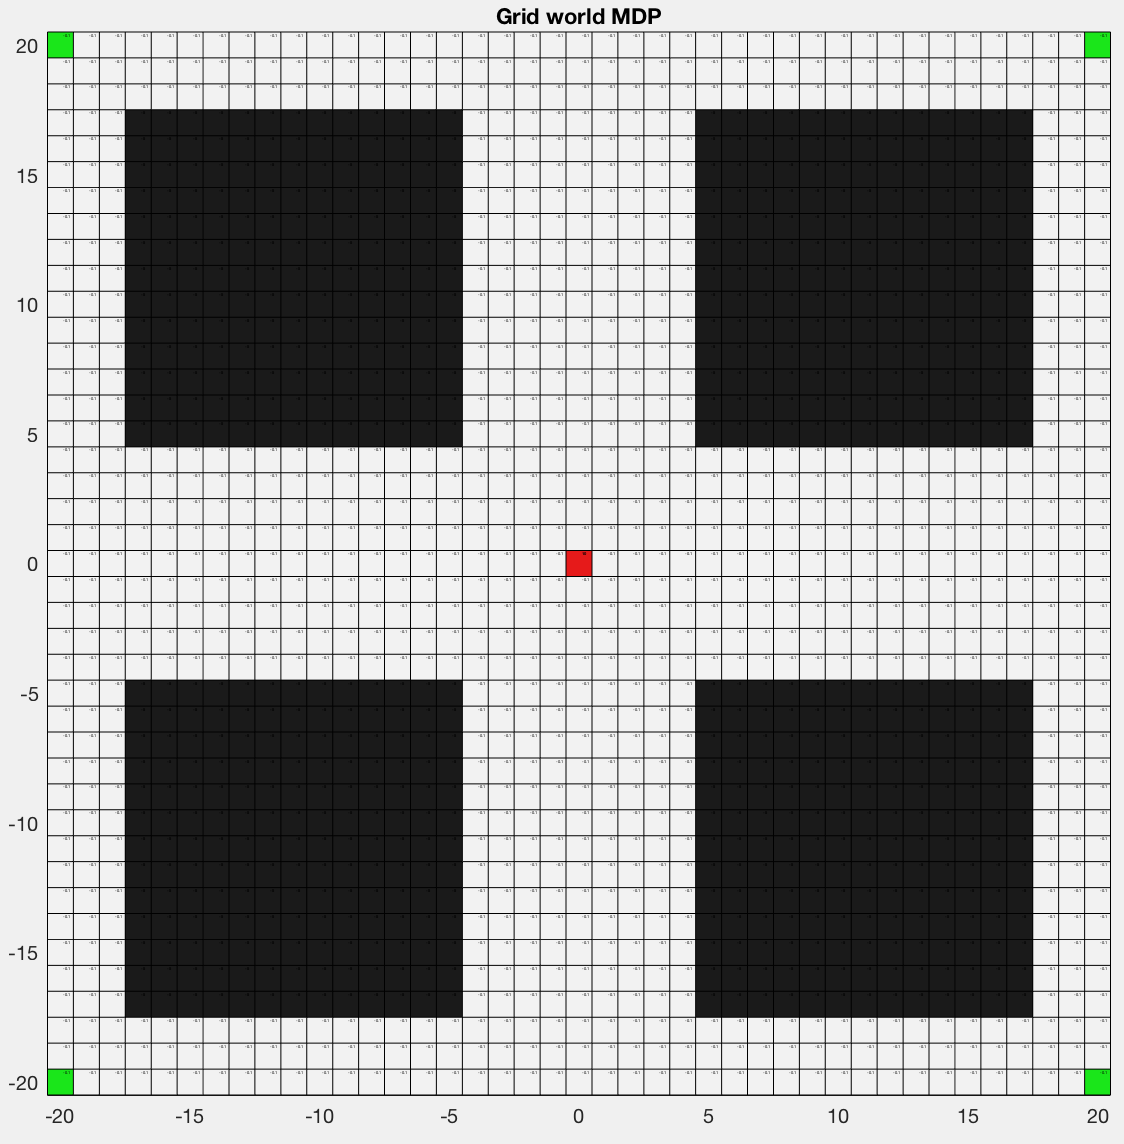
\includegraphics[width=\linewidth]{maze_grid}
					\caption{The \emph{maze\_grid} state space}
					\label{fig::maze_display}
				\end{minipage}
				\hfill
				\begin{minipage}{0.45\linewidth}
					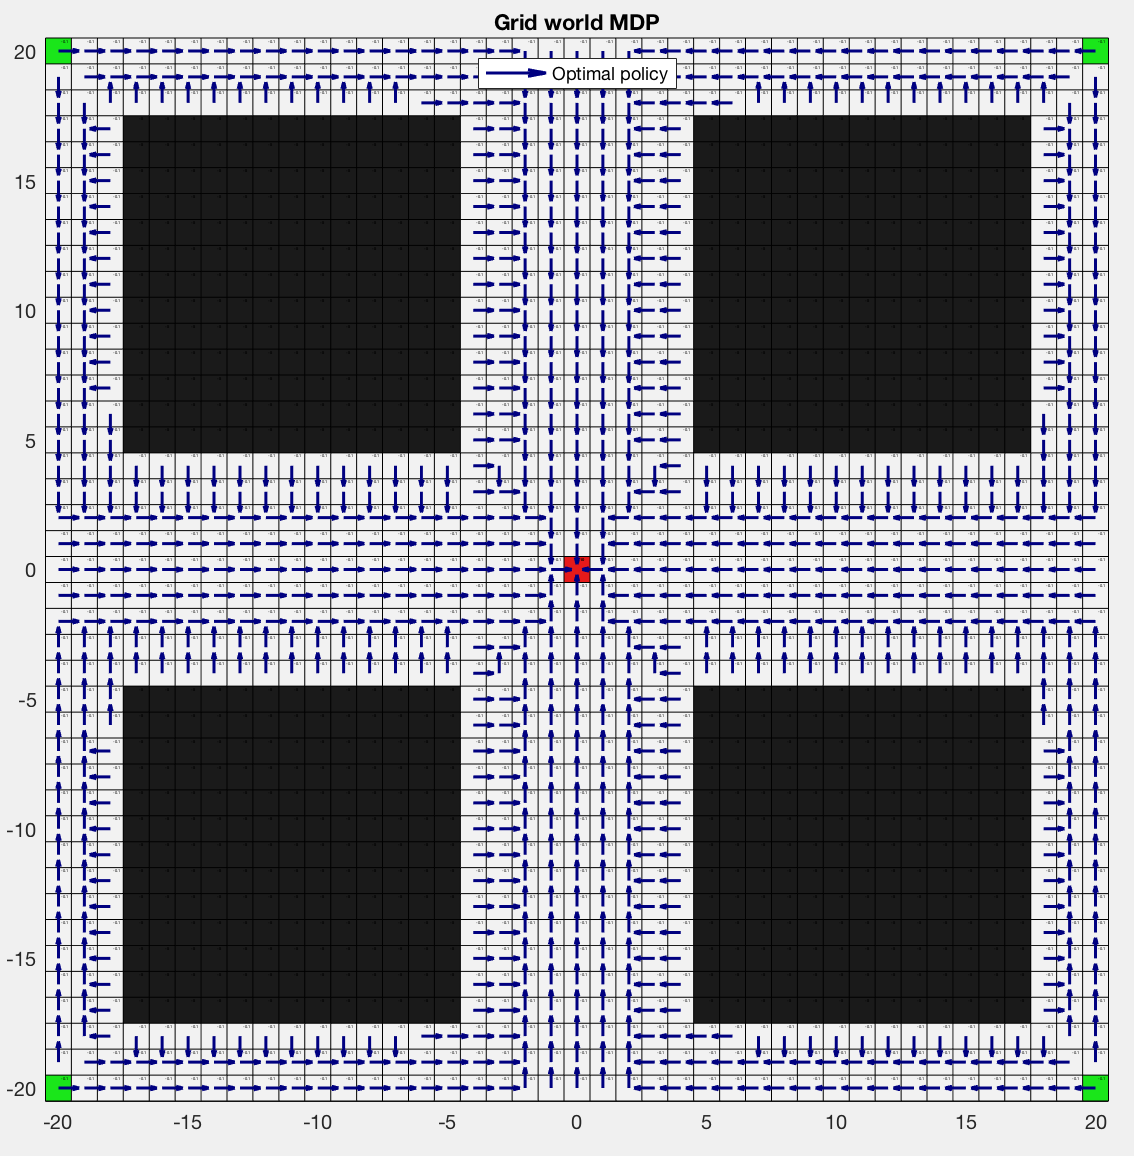
\includegraphics[width=\linewidth]{maze_optimal_policy}
					\caption{Optimal policy, computed with DP}
					\label{fig::maze_optimal_policy}
				\end{minipage}
			\end{figure}
				
			
						
			\paragraph{} Figure (\ref{fig::comp_maze}) displays the convergence (expressed as average reward on minibatch) for Qlearning, Sarsa($\lambda$), Sarsa(0) and Watkins Q($\lambda$). By average reward on minibatch, we mean that at every iteration, the reward is average around a given number of trajectories, following the same \emph{exploratory} policy. This allows to reduce the stochasticity of trajectories while learning and give a smoother estimation of how well the algorithm is learning. As a way of comparing them to the optimal and random policies, we also plot the average rewards perceived by the latest along many trajectories. \newline
For all the learning algorithms tested, we used optimistic action-value initialisation to promote exploration. This explains why many negative rewards are perceived in the beginning. 
				
			\begin{figure}
				\begin{center}
					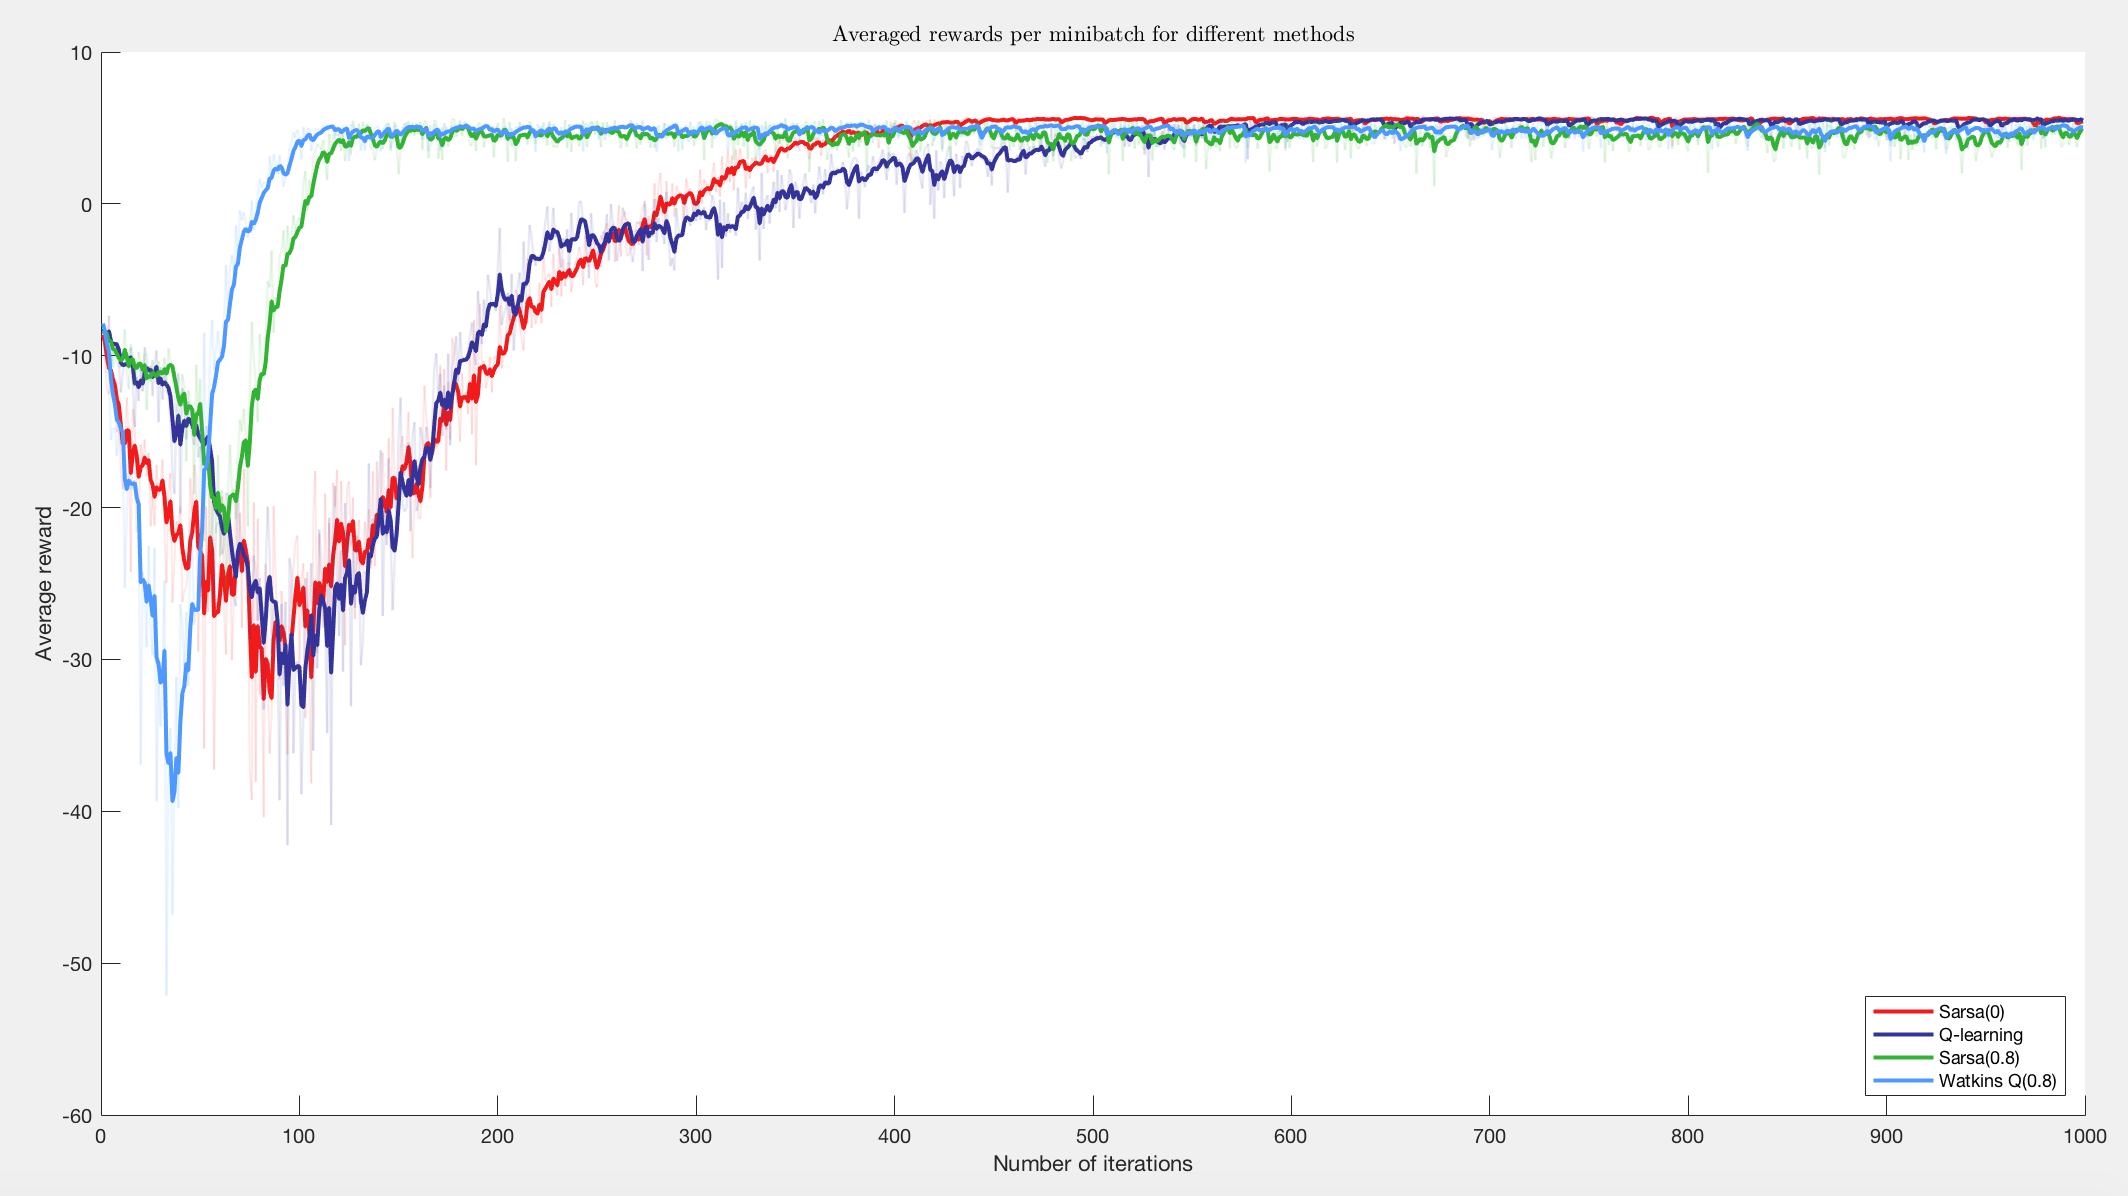
\includegraphics[width=\linewidth]{comp_maze}
					\caption{Average rewards on minibatch for learned policies, optimal policy and random policy.}
					\label{fig::comp_maze}
				\end{center}
			\end{figure}
		
			\paragraph{} As explained before, this environment is considered as a base line in all that follows, and will serve as a sandbox model where we will test our different methods for an imitation learning based approach. 
		}
		
	\section{First naive approaches}
	{
		\subsection{Constant compliance}
		{
			\paragraph{} In order to grasp as well as possible some intuition behind a compliance-based learning, we decided to first implement a really simple method, which consist in following the teacher's recommandation with a constant probability $p$ (close from $1$), defined globally (the same for all the states). More formally, the \emph{action selection} process is defined as follows. For all $s\in\mathcal{S}$ 
			\begin{equation}
				a = \left\{
				\begin{aligned}
					&a_m \, \text{with probability }p  \text{ independent of } s\\
					& a \in \mathcal{A}(s) \text{ (softmax action picking based on current Qvalues)}
				\end{aligned}\right.
			\end{equation}
			
			\paragraph{} The learning is done with a succession of action selection based on a five tuple $s,a,r,s',a'$ (the SARSA framework) and the usual TD(0) updates : $\forall s\in\mathcal{S}, a\in\mathcal{A}(s)$
			\begin{equation}
				Q(s,a) \leftarrow Q(s,a) + \alpha \left[ r + Q(s',a') - Q(s,a) \right]
			\end{equation}
			
			\paragraph{} Therefore, the learner \emph{complies} with the teacher with probability $p$, and decide to choose its own action (that \textbf{could include} $\pmb{a_m}$) with probability $1-p$. Only the action selection (hence the \emph{exploratory policy}) is impacted by the presence of the mentor. 
			
			\paragraph{} The intuition behind this approach is rather simple : we direct the exploration of the learner with the recommandations from the teacher, while still enabling it to search around them, based on its current Q-values. The softmax based exploration is regulated by a temperature factor, making it greedy in limit. 
			
			\paragraph{} The figures (\ref{fig::comp_opt_verynaive}) and (\ref{fig::comp_subopt220_verynaive}) display the learning obtained (cumulated rewards averaged over mini-batches) when fed with, respectively, the optimal policy for the MDP and a slightly suboptimal one. 
			
			\begin{figure}[h!]
				\begin{minipage}{0.5\linewidth}
					\begin{center}
						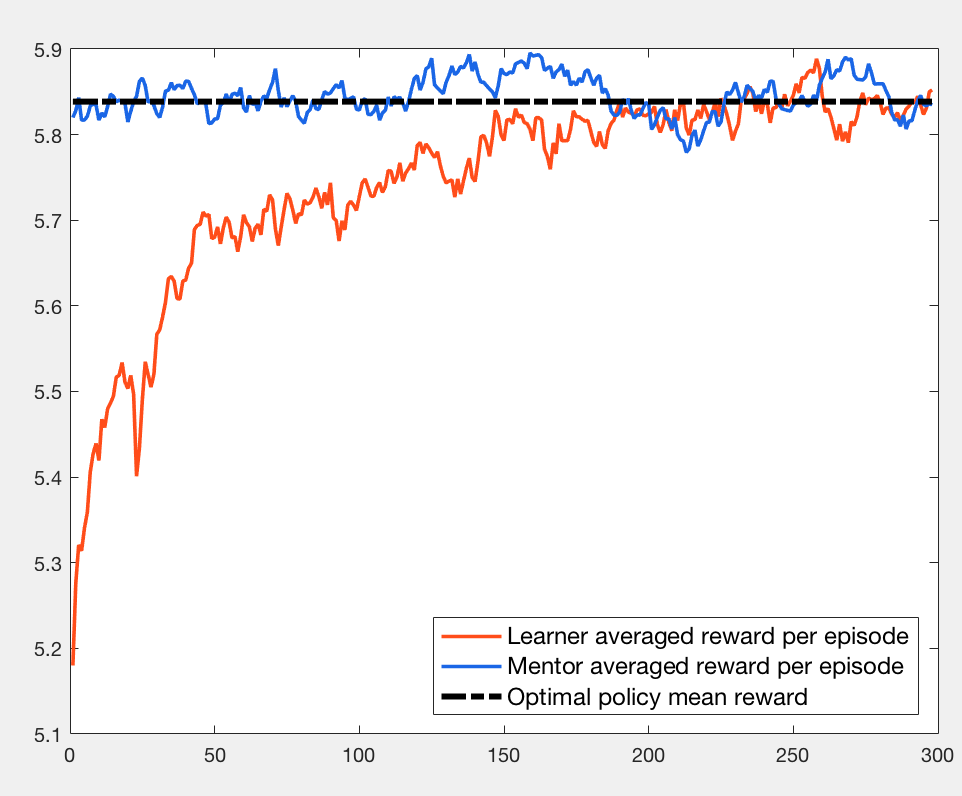
\includegraphics[width=0.9\linewidth]{very_naive_opt}
						\caption{Constant compliance learning, $p=0.9$, with the optimal mentor}
						\label{fig::comp_opt_verynaive}
					\end{center}
				\end{minipage}
				\begin{minipage}{0.5\linewidth}
					\begin{center}
						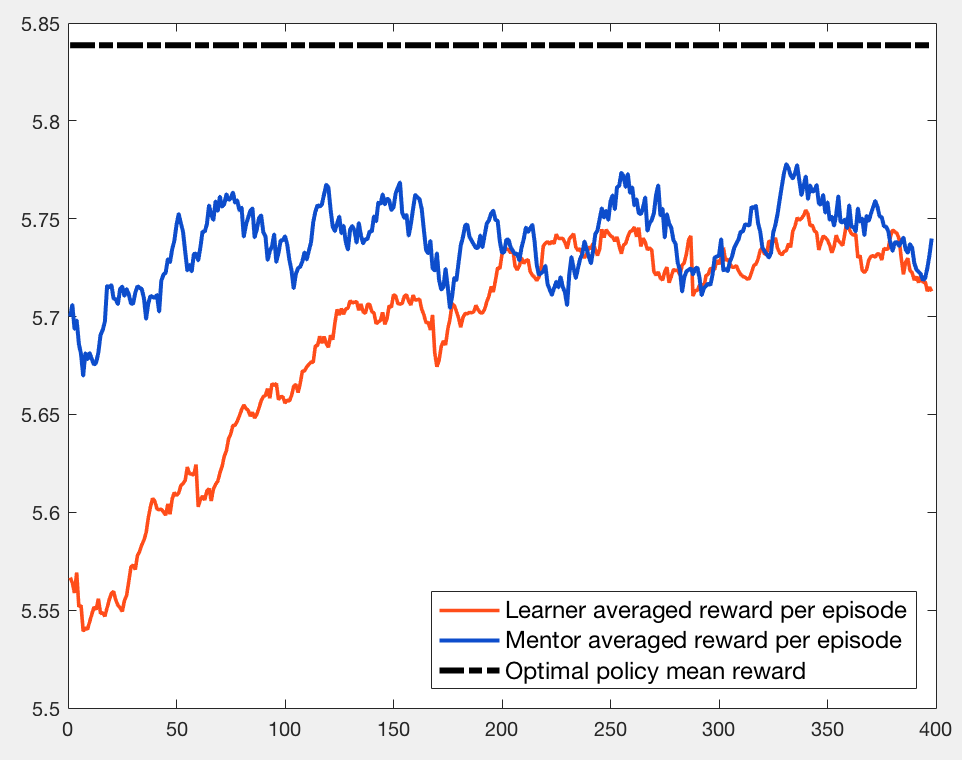
\includegraphics[width=0.9\linewidth]{very_naive_200}
						\caption{Constant compliance learning, $p=0.9$, with a slightly suboptimal mentor}
						\label{fig::comp_subopt220_verynaive}
					\end{center}
				\end{minipage}
			\end{figure}
	
			\paragraph{} Figure (\ref{fig::comp_opt_verynaive}) shows that from its exploration, the learner is able to quickly learn his way thanks to the optimal mentor. As expected, it eventually follows the mentor's action, wether it complies or not, since the recommended action holds the best action-values. On the other hand, figure (\ref{fig::comp_subopt220_verynaive}) : because of the high confidence the learner initially have in its mentor, its is never able to reach optimal performance, and the policy its renders actually mimic its mentor suboptimal one. Still, one could expect the learned policy to be slightly better than its suboptimal teacher's one, even if not optimal. However, achieving this comes with a lot of effort in the tuning of $p$ and of the softmax distribution temperature decrease coefficient. 
	
			\begin{figure}[h!]
				\begin{center}
					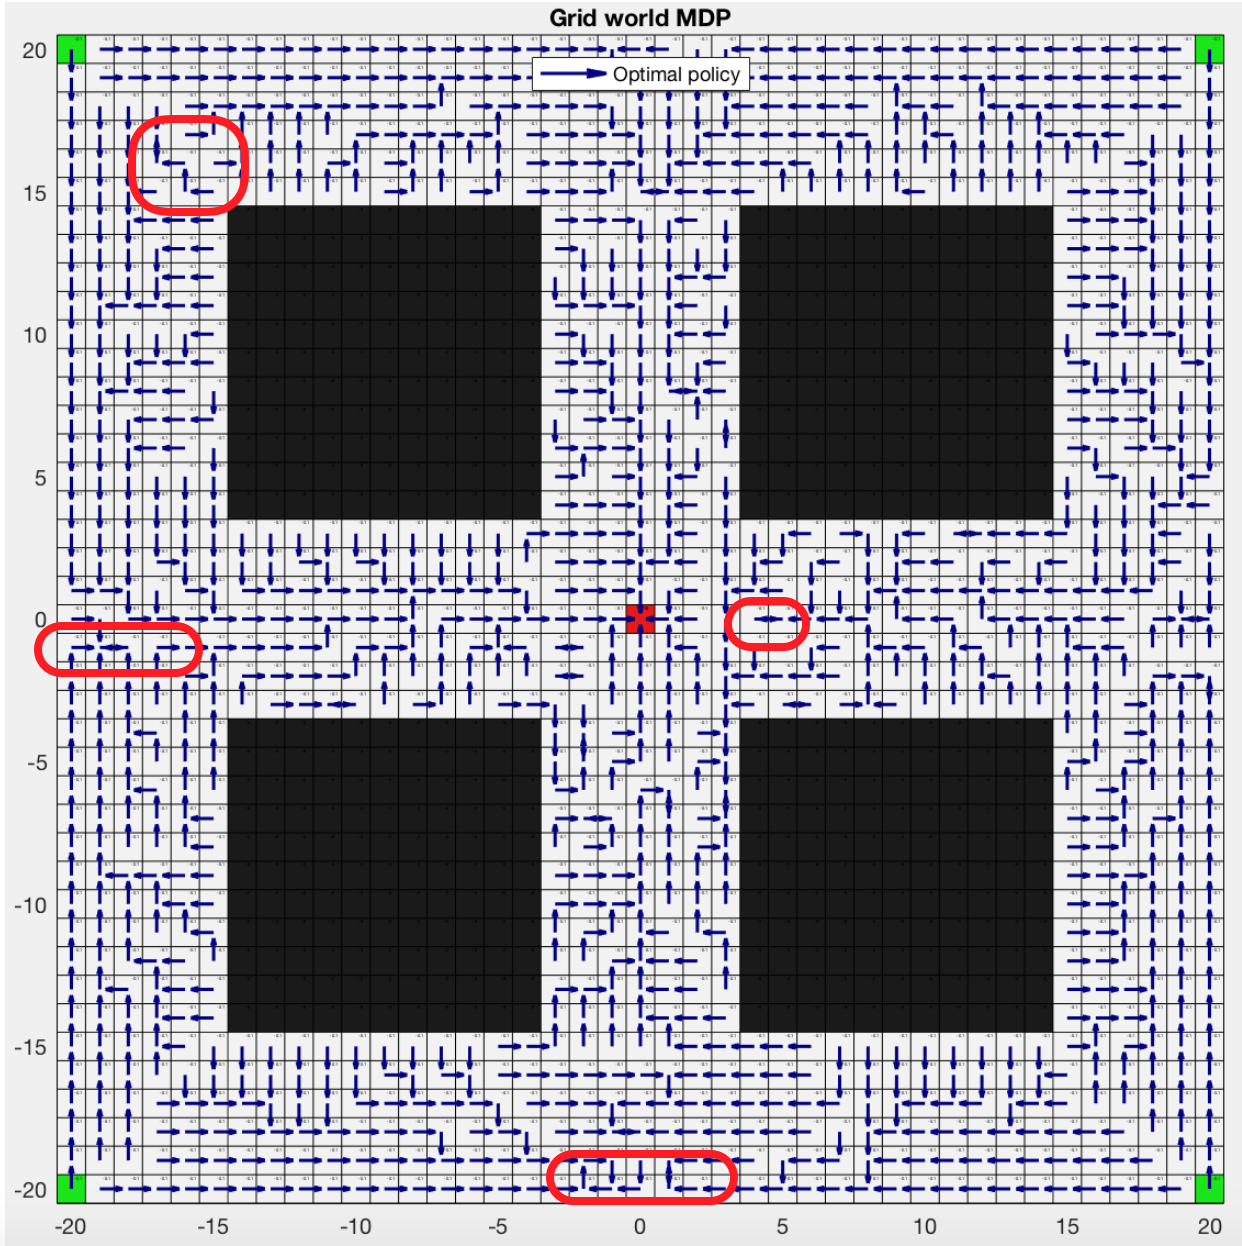
\includegraphics[width=0.7\linewidth]{subopt_policy_block}
					\caption{An exemple of suboptimal mentor policy that doesn't always lead to the positive reward}
					\label{subopt_policy_block}
				\end{center}
			\end{figure}
			
			\paragraph{} This remark actually pinpoints a major downside of this method, that is the need of fine tuning of the parameter $p$. But obviously, there is even a bigger downside, that would after become a major game killer and is related to how we generate suboptimal policies from learner. Indeed, mentor policies are taken by generating greedy policies (argmax over the Q-values) of a learner that hasn't completed its learning. Therefore, some mentors can be suboptimal enough to only show a good direction of exploitation, but not be able to reach the target. On a learning from demonstration point of view, such a phenomenon could happen if the human teacher only show the robot part of the task it has to do. Figure (\ref{subopt_policy_block}) displays such a policy, where the mentor's policy creates loops and does not always leads to the positive reward.  \newline. 
			Applying the latest method with such a teacher is fatal for the learning, as the learner discovers that following the mentor's action yields largely negative rewards, but is not able to bypass them as it keeps a constant confidence in its teacher. This leads the learner to build up low Q-values in the directions of the teacher, and trying to follow an opposite path from the mentor. This is highly counter-productive since the mentor still gives the right exploration direction. 
		
		\subsection{Constantly decreasing compliance }
		{
			\paragraph{} One of the downside of the constant compliance approach is that the exploratory behavior is always biased by the mentor's recommandation. This breaks the need of this policy to be \emph{greedy in limit} (which is a specification of the SARSA algorithm). In the case of a sub-obptimal mentor, this means that the optimal behavior could never be reached. 
			
			\paragraph{} We now decide to comply with SARSA's exigence to be greedy in limit. Therefore, $p$ is \emph{constantly decreased along the learning procedure} : 
			\begin{equation}
				p_{t+1} = \beta p_{t}
			\end{equation}
			with $\beta < 1$. As before, the temperature of the Gibb's softmax sampling also goes to $0$ as the learning goes on. 
			
			\paragraph{} The action-selection is therefore biased by the mentor's recommandation in the beginning of the learning only, and slowly decides to take its own choices, based on its current Q-values estimates. This approach sounds more promising as the learner is more likely to quickly discover the location of high rewards (following the teacher policy with $p$ close to 1), and will then makes it own exploration along those trajectory, to end up in a setting where the teacher's actions are now longer considered. 
		
					\begin{figure}[h!]
				\begin{minipage}{0.5\linewidth}
					\begin{center}
						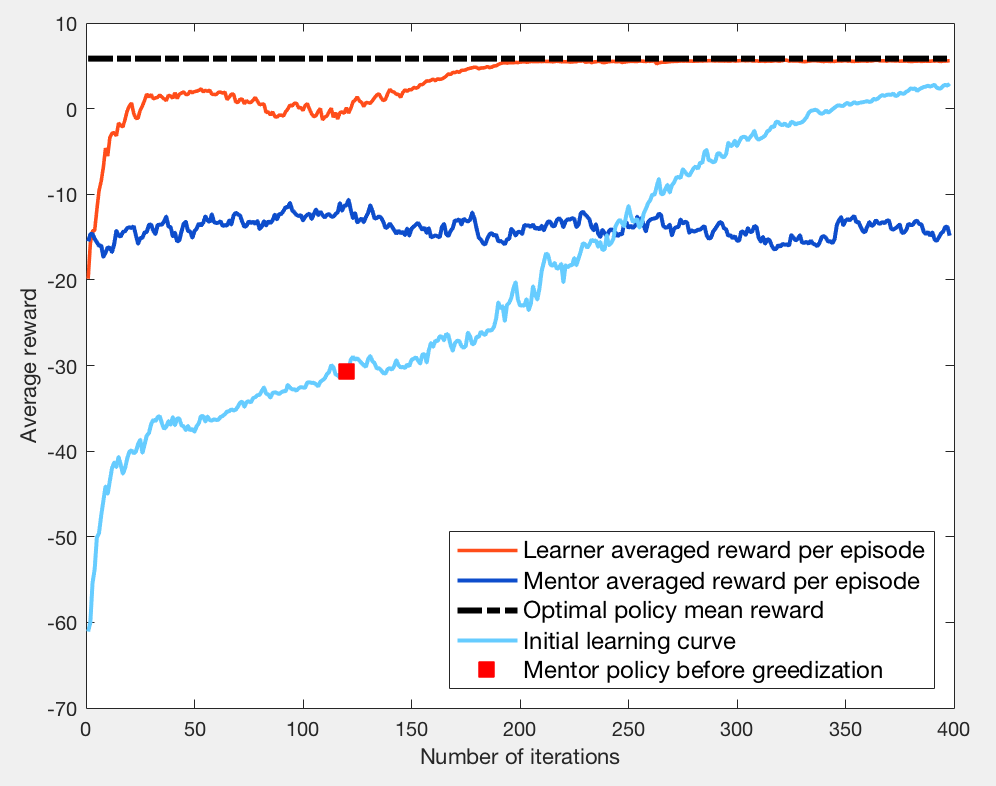
\includegraphics[width=0.9\linewidth]{comp_naive_compliance_120}
						\caption{Constantly decreasing compliance learning, $\beta = 0.99$}
						\label{fig::comp_naive_compliance_120}
					\end{center}
				\end{minipage}
				\begin{minipage}{0.5\linewidth}
					\begin{center}
						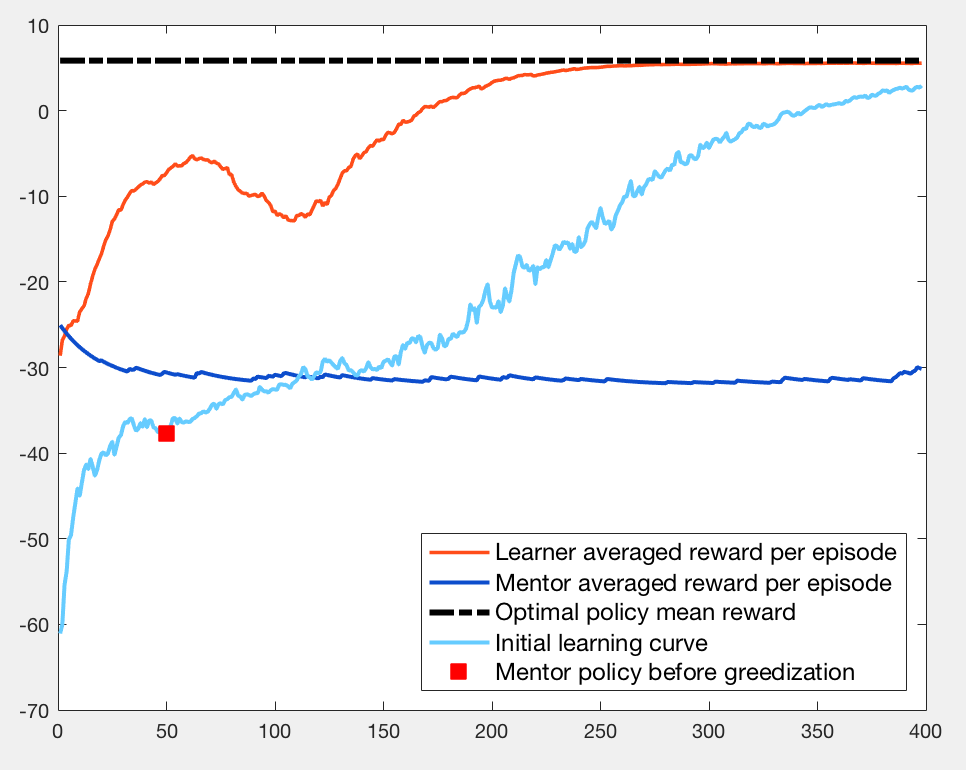
\includegraphics[width=0.9\linewidth]{comp_naive_compliance_50}
						\caption{Constantly decreasing compliance learning, $\beta = 0.97$}
						\label{fig::comp_naive_compliance_50}
					\end{center}
				\end{minipage}
			\end{figure}
			
			\paragraph{} Figures (\ref{fig::comp_naive_compliance_120}) and (\ref{fig::comp_naive_compliance_50}) display the result on two sub-optimal policies, that were derived from the Q-values learned at a given moment (denoted through a red square) in a learning process. They show that with this approach, while the learner is compliant with the teacher, it steadily increases its accumulated reward thanks to its exploratory actions, where he discard the teacher's recommandation. However, it then comes to a plateau (or even an undershoot) when the guidance by the teacher becomes too weak as $p$ reaches a critical level. The learner then mostly relies on its exploratory actions (which volatility are guided by its learning processus' temperature) to explore the space where the teacher's action never took it before. Once it has somehow learnt the action value function related to this part of its state space, and as its temperature goes down, the learner's accumulated reward goes up until it reaches the level of the optimal policy. 
			
			\paragraph{} With this technique, the learner is therefore able to learn the optimal policy even if following its teacher recommandation never takes it to the target. It is interesting to see, in such case, what policy the learner actually learns. In figure (\ref{fig::learnt_from_mentor}), we display the policy learnt from the mentor's policy showed in figure (\ref{subopt_policy_block}). One can notice that the learner actually learns to avoid place where the mentor was wrong or created loops, and forks to part of the state space where the teacher was more accurate. 
			
			\begin{figure}[h!]
				\begin{center}
					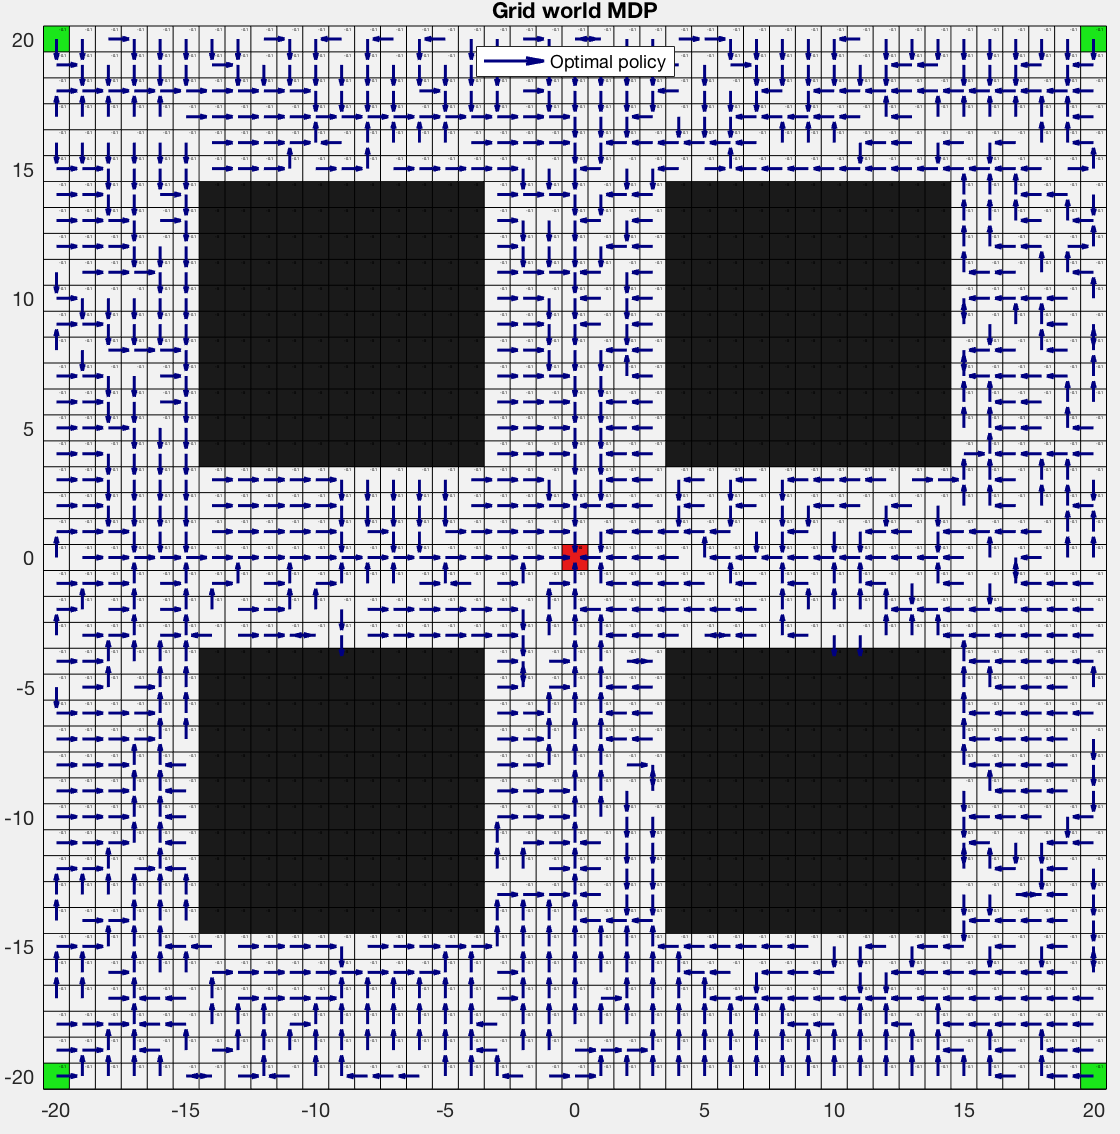
\includegraphics[width=0.7\linewidth]{learnt_from_mentor}
					\caption{Policy learnt from a suboptimal mentor}
					\label{fig::learnt_from_mentor}
				\end{center}
			\end{figure}


		}		
		
		\paragraph{} If this approach seems to work relatively well, there are still some critical downsides to it. First of all, a lot of tuning is required in order to find the hyper-parameters ($p_0$, $\beta$, temperature evolution, ..) that lead to a fast learning. Also, there is an undershoot in the learning that seems to slow it down, due to the exploring phase that happens when $p$ becomes too low.  Such exploration could be avoided or reduced if the learner is able to figure out quickly that indeed, the mentor was right in its recommandation.
		
		%% TODO : talk a bit about learning from slightly suboptimal ? 
	}
	
	\section{Adaptive compliance approach}
	{	
	
		\paragraph{} The two methods described below both have the same end goal : speed up the learning of an agent by using mentor recommandations, while overcoming eventual mentor sub-optimality.  They try to achieve that by computing \emph{exploration policies} softly related to $\pi_m$. By simplifying a lot, we can say the resulting algorithm first learn the state-value function for $\pi_m$ and then tunes its exploration policy according to wether he believes that policy to be sub-optimal, hence learning the optimal policy quicker. 
		
		\subsection{Actor-critic approach}
		{
			\paragraph{}  Let us define, for all $s\in\mathcal{S}$, $\nu(s) \sim B(p(s))$ a Bernoulli random variable where the parameter $p(s)$ is given a Beta prior : $p(s)\sim \beta(\alpha(s),\beta(s))$ and represents the trust we have in a mentor's recommandation at state $s$. 
			
			\paragraph{} At each state $s$ of its exploration trajectory, the agent is confronted with a first decision : either listen to the teacher (and follow its recommended action) or discard its recommandation and follow some other available action. This decision is sampled over the random variable $\nu$. \newline
			We will therefore perform a $\color{red}p$\textcolor{red}{\emph{-greedy policy}} with respect to the teacher recommandation : 
			\begin{equation}
				\forall s\in\mathcal{S}, \quad \pi_\nu(s) = 
					\left\{ 
					\begin{aligned}
						&a_m \text{ with probability } p \\
						& a\neq a_m \text{ with probability } (1-p)
					\end{aligned}
					\right. 
			\end{equation}
			
			\vspace{10pt}
			\noindent \textbf{Remarks}\\ 
			\vspace{3pt}
			
			\hfill
			\begin{minipage}{0.95\linewidth}
				\begin{leftbar}
						\paragraph{} \noindent $\triangleright$ The confidence we have in the teacher influence our exploration policy. The more confident we are with the mentor, the more we will perform its recommended action. On the other hand, if we think the mentor is wrong, we will perform more exploratory moves. \\
						\paragraph{} \noindent $\triangleright$ The prior on $p$ reflects our initial trust in our teacher. \\
						\paragraph{} \noindent $\triangleright$ \emph{Question} : how should we pick $p$ ? Sample it from the Beta law, or just take its expected value ($\E{p} = \alpha (\alpha + \beta)^{-1}$) ? \\
						\paragraph{} \noindent $\triangleright$ When the learner decides to discard the mentor's recommandation, it selects its action with Gibbs distribution (softmax) based on its current estimate of the remaining actions Q-values. 
				\end{leftbar}
			\end{minipage}
		
			\paragraph{} We want to, based on this exploration policy, to learn the optimal policy Q-values. We also want to learn the point-wise confidence we should have in our mentor. For any $5$-tuple $(s,a,r,s',a')$, we can compute the TD value : 
			\begin{equation}
				\delta_t = r + \gamma Q(s',a') - Q(s_t,a_m)
			\end{equation}
			which directly compares an estimated expected return of action $a$ with the current estimate of the expected return of the mentor action. Another possibility is to compute : 
			\begin{equation}
				\delta_t = \delta_t = r + \gamma Q(s',a') - \max_{a\in\mathcal{A}(s)}{\left\{ Q(s,a)\right\}}
			\end{equation}
			which should be more general as it compares the expected return for action $a$ with the best expected return possible. 
		
			\paragraph{} We then apply the following update rule to $p$ : 
			\begin{equation}
				\begin{aligned}
					\alpha &\leftarrow \alpha +  \mathds{1}_{a=a_m}\delta_t (1-\eps_t)\\
					\beta &\leftarrow \beta +   \mathds{1}_{a\neq a_m}\delta_t (1-\eps_t)
				\end{aligned}
			\end{equation}
			The intuition behind this update rule is simple : if we see that the expected return for the mentor action decreases, then we decrease $\alpha$ which results in a shift of $p$ toward a smaller confidence (and accordingly for the $\beta$ term update). \newline 
			The therm $\eps_t$ is our learning rate that can be understood as a compliance term. It starts near $1$ and decreases toward $0$ as we explore our state space. It might not be that useful because the existence of the prior should avoid overfitting to some exploration noise (especially in the beginning of the process) in most cases. 
		
			\paragraph{} The Q-values for the initial MDP are updated with SARSA algorithm, as it is usually done. Only the exploration policy is different (for instance, it will be in the usual case derived directly from the learned action function). 
		}
	
		\subsection{Action value approach}
		{
			\paragraph{} We consider here a somewhat similar approach, where our listen vs discard exploration policy is computed according to the current estimated values of the actions \emph{'listen'} and \emph{'discard'}. Let us introduce the action spaces : 
			\begin{equation}
				\forall s\in\mathcal{S}, \, \mathcal{A}_c(s) = \left\{ 'listen', \, 'discard'\right\}
			\end{equation}
			to which we assign the action values $Q_c(\cdot,l)$ and  $Q_c(\cdot,d)$ (where $l$ denotes the action of listening and $d$ the action of discarding the teacher recommendation). 
			
			\paragraph{} The exploration is done by computing a soft policy derived from $\{Q_c(s,l), Q_c(s,d)\}$ for all $s\in\mathcal{S}$. We do this using a Gibbs softmax distribution, which yields : 
			\begin{equation}
				\forall s \in\mathcal{S}, \quad \pi_c(s) = 
					\left\{
						\begin{aligned}
							&'l' \text{ with probability } p=\sigma\big(Q_c(s,l) - Q_c(s,d) \big) \\
							& 'd'  \text{ with probability } 1-p
						\end{aligned}
					\right.
			\end{equation}
			where $\sigma(\cdot)$ is the logistic sigmoid. 
			
			\paragraph{} The update rule for the initial MDP is performed as usual, using TD updates : $\forall{(s,a)}\in\mathcal{S}\times\mathcal{A}(s)$
			\begin{equation}
				Q(s,a) \leftarrow (1-\alpha)Q(s,a) + \alpha \left[ r + \gamma Q(s',a')\right]
			\end{equation}
			After each of those update, we also make the following update : 
			\begin{equation}
				\left\{
				\begin{aligned}
					&Q_c(s,l) = Q(s,a_m) \\
					&Q_c(s,d) = \max_{a\neq a_m} Q(s,a) 
				\end{aligned}
				\right.
			\end{equation}
		
			\vspace{10pt}
			\noindent \textbf{Remarks}\\ 
			\vspace{3pt}
		
			\hfill
			\begin{minipage}{0.95\linewidth}
				\begin{leftbar}
						\paragraph{} \noindent $\triangleright$ The use of the $\max\{\cdot\}$ operator is not really reflective of the policy that is used to pick an action when the learner decides not to listen to its mentor. However, since this policy is supposed to be greedy in limit, we hope this wouldn't affect the result as $t\to\infty$.. \\
						\paragraph{} \noindent $\triangleright$ \textcolor{red}{Idea} : looks a lot like hierarchical MDP .. maybe have a closer look to that theory ? 
				\end{leftbar}
			\end{minipage}
		
			\paragraph{} We can introduce some prior confidence in the teacher by setting, $\forall s\in\mathcal{S}$ : 
			\begin{equation}
				Q^0_c(s,l) - Q^0_c(s,d) = \log\{\frac{p}{1-p}\}
			\end{equation}
			where $p$ is the retained probability of initially choosing to listen to the teacher. 
			}
		}	
	}
	
	\chapter{Results}
	{
	
	}
	
	\chapter*{Conclusion}
	\addcontentsline{toc}{chapter}{Conclusion}
	
	
	\bibliographystyle{alpha}
 	 \bibliography{bibfile}
	 \nocite{*}
  
\end{document}